\documentclass{cls/ma-ths}

%------------------------------------------------------------------------
% Preamble setup
%------------------------------------------------------------------------
% Paket für Bibliographie im APA-Stil
% \usepackage[sort&compress]{apacite} % remove or comment this out
\usepackage[backend=biber, style=apa]{biblatex} % loads APA style with biber
\addbibresource{ref.bib} % add your bibliography file

% Ermöglicht das Setzen von Float-Barrieren zum Erzwingen von Einbettungen (Tabellen, Figures)
\usepackage{placeins}

% Hyperlinks im Dokument
\usepackage{hyperref}

% Verarbeitung von URLs
\usepackage{url}

% Für professionelle Tabellen
\usepackage{booktabs}

% Blackboard Math Symbole (AMS)
\usepackage{amsfonts}
\usepackage{amsmath}
\usepackage{amssymb}

% Kompakte Symbole für Brüche wie 1/2
\usepackage{nicefrac}

% Mikrotypografie-Optimierungen
\usepackage{microtype}

% Kopfzeilen- und Fußzeileneinstellungen (wird vom springer template benötigt)
\usepackage{fancyhdr}

% Einbindung von Grafiken
\usepackage{graphicx}
\usepackage{tabularx}
\usepackage{float}
\usepackage{rotating}
\usepackage{placeins}
\usepackage{comment}

% Wegen Font Shape not available hinweisen
\usepackage{anyfontsize}

% Pfad zu den Grafiken festlegen
\graphicspath{ {.} }

% Für Algorithmen und Pseudocode
\usepackage{algorithm}
\usepackage{algpseudocode}

% Für Absätze ohne Einrückung (\\ wird nicht meht benötigt)
\usepackage{parskip}


%Dieser Befehl beeinflusst das vertikale Layout des Dokuments. Standardmäßig versucht LaTeX, die Seiten so zu formatieren, dass der Text gleichmäßig über die Seiten verteilt ist, wodurch jede Seite die gleiche Höhe hat (was zu "vollen" Seiten führt). Der Befehl \raggedbottom bewirkt, dass LaTeX diese automatische Verteilung nicht anwendet und stattdessen den Seiteninhalt so belässt, wie er ist, auch wenn dies bedeutet, dass einige Seiten kürzer sind als andere.
\raggedbottom
\makeglossaries
\loadglsentries{glossary} % glossary.tex is in the project root folder
% Comment out glsaddall to avoid adding all entries in development phase
% This ensures only referenced abbreviations are included
%\glsaddall  % Ensure all glossary entries are added

\begin{document}

%------------------------------------------------------------------------
% Front Matter
%------------------------------------------------------------------------
\frontpage
\cleardoublepage
\thispagestyle{empty}
\null
\cleardoublepage
% Front page logic in cls/ma-ths.cls
% Description: Contains the abstract of the thesis.
\thispagestyle{plain}

\vspace*{1.5in}

\begin{center}
  {\Large \textbf{Abstract}}
\end{center}

This thesis addresses the validation of automatically generated simulation-based digital twins within discrete material flow systems. While generating simulation-based digital twins from data promises reduced creation and updating efforts, these benefits are negated if verification, validation, and uncertainty quantification (VVUQ) require manual expert involvement. To overcome this, a multi-layered, automated VVUQ framework is developed and empirically validated. This framework integrates data processing using object-centric event logs, twin synchronization, and machine learning-based validation via a supervised classification approach. Results from a conducted case study demonstrate that a Bidirectional Long Short-Term Memory-based classifier effectively identifies statistically significant differences between real and simulated process data, yielding consistently high rejection rates and highly significant p-values ($p \ll 0.01$) in permutation tests across multiple simulation-based digital twin components (process flow, resource allocation, time models). The framework enables continuous, automated validation, offering a scalable and objective alternative to periodic manual checks and providing feedback for targeted simulation-based digital twin improvement. While requiring initial infrastructure setup efforts, the methodology contributes a practical approach for enhancing simulation-based digital twin reliability and trustworthiness in manufacturing.

\vspace{0.3in}

\textbf{Keywords:} Simulation-based digital twin, Automated verification, validation, and uncertainty quantification, Data-driven validation, Object-centric event log, Machine learning, Permutation testing, Discrete material flow systems, Manufacturing systems, Process mining.

\clearpage
\tableofcontents
\clearpage
\clearpage
\addcontentsline{toc}{chapter}{List of Tables}
\listoftables
\clearpage

\clearpage
\addcontentsline{toc}{chapter}{List of Figures}
\listoffigures
\clearpage

%------------------------------------------------------------------------
% Glossary
%------------------------------------------------------------------------
\printglossary[type=\acronymtype, title={List of Abbreviations}]

%------------------------------------------------------------------------
% Main Chapters
%------------------------------------------------------------------------
\chapter{Introduction}
\label{chap:introduction}

\section{Initial Situation}
Digital Twins (DT) are a key technology at the front of the fourth industrial revolution, coined Industry 4.0.
The latter term is characterized by the interaction of cyber-physical systems (CPS), the Internet of Things (IoT), and cloud computing to create smart factories with the goal of automation and efficiency \parencite{Oztemel2020}. Companies pursue this ideal by trying to remain competitive through the adoption of innovative technologies that promise enhanced productivity and reduced operational costs. One such technology that supports this transformation is the DT. It can be defined as a virtual representation of physical assets enabling real-time monitoring and optimization \parencite{Tao2018ijamt}. The DT bridges the connection between the two entities with a bi-directional data flow to exchange information and to influence the behaviour of the physical asset \parencite{grieves2014digital}. This technology in Industry 4.0 connects the physical and digital worlds through real-time data integration, simulation, and optimization \parencite{judijanto2024trends}.

Although this field is rapidly evolving, a unified definition of DT has yet to be established due to the diverse requirements and perspectives across different fields. In engineering, the focus might be on the real-time interaction between physical systems and their digital counterparts, whereas in computer science, the emphasis is often on data integration and simulation capabilities. These varying priorities result in multiple interpretations and applications of the term DT. The term was first introduced by Michael Grieves in 2002, defining it as a digital representation of a physical object or system \parencite{grieves2014digital}. However, the concept has evolved since then, encompassing a broader range of applications and technologies. Going back through the literature, there are three terms used to describe similar characteristics of DT: Digital Model (DM), Digital Shadow (DS), and Digital Twin (DT), see \Cref{fig:Kritzinger} \parencite{jones2020characterising,Zhang2021jmsy}.

\begin{figure}[htbp]
  \centering
  \includegraphics[width=0.8\textwidth]{figures/kritzinger.png}
  \caption{Comparison of Digital Shadow (DS), Digital Model (DM) and Digital Twin (DT) as presented by Kritzinger (2018). This distinction is crucial for understanding validation requirements across different digital representation types.}
  \label{fig:Kritzinger}
\end{figure}

The DM represents the most basic form. It contains manual data connections between physical and digital entities. These connections can be temporarily shifted or even disconnected. There is no control of the digital object over the physical entity. It rather is a simple or complex model \textit{describing} the modelled object. It can not make decisions by itself to influence the physical object. The reason lies in the potential outdated data the digital part possesses or in the fact that it does not contain logic to control the data flow back to the physical part by itself. The control and the obligation to interpret the results is completely in the hands of the modeller.
The DS is a more advanced version of the DM. It is a digital representation of the physical object, which is continuously updated with real-time data. The DS can be used for monitoring, analysis and simulation purposes. It can predict the future state of the physical object based on the current state and historical data. However, the DS is not able to influence the physical object. The control is, similar to the DM, still in the hands of the modeller. A DS is frequently used for simulation purposes and is often misclassified as a DT in the literature \parencite{kritzinger2018digital,buildings11040151}.
The DT is the most advanced version of the triplet. It is a digital representation of the physical object, which is also continuously updated with real-time data. The DT can be used for monitoring, analysis, and \textit{control} purposes. It can predict the future state of the physical object based on the current state and historical data. The DT can also influence the physical object by sending control signals to it. The control is partially or completely in the hands of the DT. The DT thus \textit{can} serve more purpose than modelling or simulating the physical object. It may serve as an autonomic system, updating itself or by help of the modeller \parencite{kritzinger2018digital}.

DTs are applied across various sectors, including manufacturing, defense, automotive, service, finance and healthcare \parencite{Tao2018ijamt}. Manufacturing stands out due to its high potential for process optimization and automation. This thesis focuses on the latter, particularly discrete material flow systems (DMFS). These systems process discrete objects (parts) that move along transportation routes or conveyor lines—either at regular or irregular intervals—integrating both production and logistics operations \parencite{arnold2005materialfluss, schwede2024learning}. A core simplification in their modeling is the abstraction of material flow as a sequence of discrete events, in accordance to the principles of discrete-event simulation (DES) \parencite{kovacs2016mathematical, robinson2014simulation}. DES is particularly well-suited for analyzing complex systems where state changes occur at discrete points in time, such as arrivals, departures, and processing steps \parencite{robinson2014simulation}.

In hindsight, DM played a crucial role in the design, planning, and control of DMFS, primarily through applications such as material flow simulations, logistic assistance systems, and digital factory implementations \parencite{Thiede2013}. However, advancements in both DS and DT have enabled a revolution from isolated, usecase-specific models toward complete digital representations that span the entire lifecycle of DMFS \parencite{Abdoune2023}. This transition is largely driven by the increasing demand for predictive capabilities by stakeholders and automated decision support in manufacturing systems, reflecting the cornerstones of Industry 4.0 \parencite{frank2019industry}. A second driver of DT innovation lies in the widely available data from IoT devices and sensors. Unlocking these potentials in model training and real-time adaption of the DT is crucial for its modelling capabilities \parencite{Tao2018ijamt}.

In practice, the automated data transfer between the digital model and the physical system is of secondary importance for DMFS management. Unlike in time-critical applications, human decision-makers remain an integral part of the control loop, ensuring that real-time automation is not always necessary \parencite{schwede2024learning}. Consequently, for this thesis, digital simulations and DTs will be treated as equivalent concepts.

Beyond merely replicating the current state and managing historical data, DTs serve a crucial function in predicting system behavior and evaluating potential modifications. The widespread adoption of DES within digital twins highlights the central role of simulation-based digital twins (SBDT) in DMFS \parencite{Lugaresi2021aifac}. As \citeauthor{schwede2024learning} emphasize, SBDTs provide decision support for optimizing cost and performance in highly competitive manufacturing environments. While current SBDTs are primarily developed and updated manually by domain experts, emerging research explores how machine learning (ML) can enhance predictive accuracy and automate model updates by automatically learning model characteristics, reducing costs and development time.

Thus, the progression from digital models to simulation-based DTs reflects an ongoing shift towards data-driven, predictive, and increasingly automated representations of DMFS, ensuring more informed decision-making throughout the whole system lifecycle \parencite{boschert2016digital,lim2020state}.

\section{Problem}
Despite the transformative potential of DT, their implementation can be challenging. The creation and maintenance of accurate DTs require substantial investments in technology and domain knowledge. This investment yields no return if the resulting model fails to accurately represent the modelled entity or delivers incorrect results. Automatic generation may be an elegant solution, but possesses the risk of overfitting or biased predictions \parencite{gemanbias}. Manufacturing data used as training data must be preprocessed and cleaned rigourusly. The DT per definition has to be able to perform real-time decision making without excessive time lags \parencite{buildings11040151}. This yields the requirement to extract, transform, clean and load (ETL process, \cite{vassiliadis2002conceptual}) data on the fly. ETL needs to happen fully in cache or memory so that inference can happen instantly. All other persistence methods would lead to excessive disk I/O \parencite{mandala2024etl}.
All these hurdles are challenges to automatic learning \parencite{ribeiro2016should,zhao2024data}. As industries integrate DT into their production processes, establishing trust becomes fundamental as well \parencite{trauer2022digital,arrieta2020explainable}. To gain widespread acceptance under coworkers, stakeholders and investors, the technology must demonstrate accuracy, transparency, and cost-efficiency \parencite{Wright2020amse,Shao2023mfglet}. Without these qualities, organizations will likely fall back to familiar methods, potentially building resistance to technological advancement \parencite{lapointe2005multilevel}. If DTs dont live up to the expectations, divestments will follow \parencite{cognizant2020divestitures}.

Even if DT learning is successfully performed, questions regarding its correctness, precision, and robustness remain unanswered. These questions are tackled by validation, verification and uncertainty quantification frameworks (VVUQ) \parencite{sel2025survey}. Ensuring the validity, reliability, and accuracy of a DT is critical, yet traditional V&V approaches rely heavily on manual expert involvement and case-specific reference values \parencite{Bitencourt2023,hua2022validation}. This creates inefficiencies, particularly in the context of automated DT generation, where such manual processes conflict with the goal of reducing development effort. \citeauthor{hua2022validation} even argue that there are no robust and standardized VVUQ methods for DTs. One hurdle to standardized VVUQ frameworks is the lack of a clear definition for validity and verification in the context of DTs \parencite{Bitencourt2023}.

For discrete material flow systems, these challenges are even more pressing due to their processual nature and stochasticity. Manufacturing processes may fail due to, among other factors, anomalies, resource constraints, software faults or human error \parencite{chenganomalies}. VVUQ approaches have to anticipate these risks. When DTs for these systems are generated automatically, conventional validation approaches become problematic, as they negate much of the efficiency gained through automation. This creates a fundamental conflict: While automated DT generation reduces initial development- and updating efforts, it simultaneously increases the complexity of validation and verification, potentially counteracting its intended efficiency gains.

\section{Objective}

The thesis thus addresses this contradiction by developing a data-driven framework for automated VVUQ of automatically generated, simulation-based DTs which have been learned from data. The focus lies on DMFS due to their practical relevance and dynamical, processual nature. The endeavor can further be concretized by the following research questions (RQ):

\begin{itemize}
  \item \textbf{RQ1:} How can automated validation and verification processes for DTs be efficiently implemented to maintain both accuracy and computational feasibility?
  \item \textbf{RQ2:} Which data-driven approaches are best suited to identify discrepancies between simulated behavior and real operational data in discrete material flow systems?
  \item \textbf{RQ3:} To what extent does the developed framework improve the quality and reliability of DTs compared to traditional V&V methods?
\end{itemize}

This thesis addresses these questions by proposing that object-centric event logs—the same data structures often used to generate DT in manufacturing—can serve as the foundation for an automated, use case-independent validation and verification framework. Such an approach would maintain the efficiency benefits of automated generation while ensuring the resulting DTs meet necessary standards. The development and monitoring of generic, statistically grounded reference values is a key aspect of this approach. Such key indicators need to have an underlying distribution and have to be quantifiable. The framework will be evaluated using a case study from the discrete material flow domain, providing empirical evidence of its effectiveness in improving model accuracy and efficiency.

\section{Structure and Methodology}

\subsection*{Structure}
The thesis is structured into eight chapters.
\Cref{chap:theory} establishes the theoretical groundwork. It begins with broad, domain-specific concepts and progressively narrowing the focus to the core topics of this thesis: Automated verification and validation (VVUQ) of simulation-based digital twins (SBDTs) in discrete material flow systems.
\Cref{sec:material-flow} introduces material flow planning and simulation, outlining the fundamental elements of production systems, including processes, resources, and control mechanisms. It defines key performance indicators (KPIs) that are essential for evaluating both real and simulated systems, thereby providing the practical context in which digital twins operate.
\Cref{sec:digital-twin} then transitions to the DT concepts. A framework for comparing DTs by \textcite{schwede2024learning} is presented. Particular attention is given to data-driven digital twins and their subset, automatically generated digital twins (AGDTs). The section concludes by contrasting AGDTs with classical simulation models, emphasizing the challenges posed by automatically generated models.
Building on this foundation, \Cref{sec:object-centric-event-logs} presents the principles of process mining (PM) and event log analysis, with a focus on object-centric event logs as a data basis for automated validation. This section demonstrates how PM acts as a bridge between real-world process data and model validation, thus enabling continuous verification of SBDTs.

\Cref{sec:vvuq-sbdt} narrows the focus further to VVUQ in the context of SBDTs, beginning with a historical overview of VVUQ methodologies. It then addresses the specific challenges posed by automatically generated models, such as data dependency and lack of transparency in model creation. The section introduces machine learning-based approaches for VVUQ, particularly classification methods for model deviation detection. It also explores the current state of VVUQ in corporate practice, emphasizing the necessity for continuous and automated validation processes.

\Cref{chap:methodology} outlines the methodology used to develop the proposed framework. It begins with a classical requirements analysis, deriving functional, technical, and data format requirements from theoretical findings. The chapter elaborates on the data-based validation strategy, machine learning-based validation approach, metrics for model evaluation, and online validation with continuous monitoring.

\Cref{chap:implementation} presents the framework implementation, starting with the architecture and system setup, followed by detailed descriptions of event log processing, simulation integration, and the machine learning pipeline.

\Cref{chap:case-study} presents the case study results, evaluating the framework's effectiveness in improving DT quality. It describes the application scenario and data basis, the automatically generated DT, validation experiments, and result interpretation. It concludes with a comparison to manual validation methods.

\Cref{chap:discussion} discusses the implications of the results and provides recommendations for future research. It evaluates the framework in light of the research questions, examines the significance of verification in automatically generated DT, addresses limitations, and explores implications for research and practice.

\Cref{chap:conclusion} concludes the thesis by summarizing key findings and their implications. It addresses the research questions and hypotheses, discusses the results' significance, acknowledges limitations, and provides recommendations for future work.

\subsection*{Methodology}

Methodologically the thesis follows a design science research approach (DSR). This approach is characterized by the development of artifacts to solve practical problems \parencite{hevner2004design,peffers2007design}. Artifacts in the sense of DSR are created objects or constructs which adress the given problem and contribute in direction of both theory and practice. The artifacts are evaluated in a real-world context to demonstrate their effectiveness. The thesis follows DSR by applying the cyclical DSR model, see figure \ref{fig:DSR}.

\begin{figure}[htbp]
  \centering
  \includegraphics[width=0.8\textwidth]{figures/dsr.png}
  \caption{The cyclical design science research model. The model consists of six steps. The problem identification (1) refers to the research gap in automated VVUQ of SBDT. Defining the solution objectives (2) specifies the research gap by formulating questions and hypotheses based on the theoretical foundations. The design and development (3) phase includes the development of the framework. The demonstration (4) phase shows the application of the framework in a case study. The evaluation (5) phase assesses the effectiveness of the framework. The communication (6) phase concludes the research by presenting the results.}
  \label{fig:DSR}
\end{figure}

The research paradigm of the thesis can be characterized as deductive-theory critical \parencite{eberhard1987einfuhrung}. A conceptual VVUQ framework is developed based on existing theoretical foundations, while deriving new requirements thorugh a requirements analysis. The framework is then applied in a case study to evaluate its effectiveness. The research is critical in the sense that it aims to improve the efficiency and effectiveness of VVUQ for automatically generated DTs. Elements of empirical research are included through the case study and the data-driven approach.


\chapter{Theoretical Foundation}
\label{chap:theory}

\section{Material Flow Planning and Simulation}
\label{sec:material-flow}
\subsection{Basic Concepts}
% Content goes here
% - Basic concepts

\subsection{Processes and Resources}
% Content goes here
% - Processes and resources

\subsection{Production Planning and Control}
% Content goes here
% - Production planning and control

\subsection{Relevant KPIs and Metrics}
% Content goes here
% - Relevant KPIs and metrics (→ Reference to 4.4: Metrics for model evaluation)

\section{Process Mining and Event Logs}
\label{sec:process-mining}

\subsection{Core Concepts}
% Content goes here
% - Standard formats and their importance for automated validation
% Standards aus Will van der Aalst Buch beschreiben die hier einschlägig sind

\subsection{Object-Centric Event Logs as a Data Basis}
\label{sec:object-centric-event-logs}
% Content goes here
% - Object-centric event logs as a data basis (→ Reference to 4.2: Data-based validation strategy)


\subsection{Process Mining as a Bridge between Process Data and Model Validation}
% Content goes here
% The importance of PM for model validation VVUQ
% - Process mining as a bridge between process data and model validation (→ Reference to 3.3)

\section{Digital Twin: Definition and Concepts}
\label{sec:digital-twin}
\subsection{Types of Digital Twins}
% Content goes here
% - Types of digital twins

\subsection{Data-Driven Digital Twins}
% Content goes here
% - Data-Driven Digital Twins (→ Reference to 3.2: Automatic model generation)

\subsection{Automatically Generated Digital Twins}
% Content goes here
% - Automatically generated digital twins
\subsection{Definitions and Differences from Classical Simulation Literature}
% Content goes here

\section{VVUQ in the Context of Simulation-Based Digital Twins}
\label{sec:vvuq-sbdt}


\subsection{Historical Development of VVUQ Concepts}
% Content goes here
% - Historical development of V\&V concepts (→ Reference to 1.2)

\subsection{Peculiarities of Automatically Generated Models}
% Content goes here
% - Peculiarities of automatically generated models (→ Reference to 3.1 and 7.2)

\subsection{Theoretical Argumentation for Merging Verification, Validation and Uncertainty Quantification}
% Content goes here
% - Theoretical argumentation for merging verification, validation and uncertainty quantification

\subsection{Machine Learning-based approaches}
% Content goes here
% Classification methods for the detection of model deviations (→ Reference to 4.3)
% Challenges in data preparation and feature selection
% Discussion of previous ML approaches in the context of the V&V problem (→ Reference to 2.2 and 4.3)

\subsection{VVUQ in the Context of Digital Twins}
% Manual vs. automated approaches
% Critical discussion of existing V&V definitions and methods (→ Reference back to 2.2)
% Challenges in the validation of automatically generated models

\subsection{VVUQ in Corporate Practice}
% Content goes here
% - V\&V as a continuous process (→ Reference to 4.5: Online validation)




\chapter{Framework Design}
\label{chap:methodology}
This chapter develops the methodological approach for automatically performing VVUQ for automatically generated SBDT in the manufacturing domain. The foundational methodology uses data-driven frameworks and applies ML tecniques to verify and validate the SBDT. The following chapter structure derives requirements besides the identified key requirements given in \autoref{sec:requirements-automatically-generated-models}, categorizes them and presents a conceptual blueprint. It is based on the theoretical findings from Chapter \ref{chap:theory} and designed to ensure that the VVUQ process is systematic, reproducible, and adaptable to different use cases.

\section{Requirements Engineering}
A thorough analysis of the requirements for the proposed VVUQ framework is essential. \Autocite{sindhgatta2005functional} distinguishes between functional (FR, \autocite{van2001goal}) and non-functional requirements (NFR, \autocite{glinz2005rethinking}). Functional requirements define the specific functions and features that the system must provide, while non-functional requirements specify the quality attributes, constraints, and performance criteria that the system must meet. Additionally, technical requirements (TR) and operational requirements (OR) may also be considered. TR specifies the technical specifications of the system which are necessary to meet the functional requirements \autocite{chikh2012new}, while OR outlines the operational constraints and conditions under which the system must operate \autocite{incose2023incose}.

The following \autoref{fig:requirements} summarizes the key requirements identified in \autoref{sec:requirements-automatically-generated-models} and adds requirements which have been derived from the theoretical findings in Chapter \ref{chap:theory}.

\begin{figure}[htbp]
  \centering
  \includegraphics[width=0.8\textwidth]{figures/req.png}
  \caption{Key Requirements for the VVUQ framework differentiated by FR, NFR, TR, and OR. }
  \caption*{Source: Own illustration.}
  \label{fig:requirements}
\end{figure}

Real-time data integration enables continuous synchronization between physical processes and the digital twin through real-time data streams. This is crucial for ensuring that the digital twin accurately reflects the current state of the physical system. The latency in this regard has to be minimized \autocite{li2018learning}. Of course, one FR has to be the Automatic VVUQ of the SBDT with its functional capabilities anomaly detection \autocite{pang2021deep}, uncertainty quantification \autocite{sel2025survey}, and adaptive recalibration to new physical states. The framework should also include an alarm management system that generates alerts and recommendations for action in the event of anomalies or validation errors. This is essential for ensuring that operators can respond quickly to potential issues and maintain the integrity of the system. The performance evaluation of the framework should be automated and include key performance indicators (KPIs) such as F1-Score, MAE, and synchronization accuracy see \autoref{sec:metrics}.

The NFRs include dynamic scalability, which allows the framework to handle large amounts of data and complex models in real time \autocite{leskovec2020mining}. This is essential for ensuring that the system can adapt to changing conditions and requirements also defined by evolving technical requirements or new demands of the stateholders. The framework should also be robust against uncertainties, meaning it should be able to tolerate noise, incomplete data, and model uncertainties like concept drift. Security is another important NFR, as the framework must ensure the confidentiality and integrity of sensitive data. Interoperability with existing systems such as MES, ERP, and PLM systems is also crucial for successful integration into existing workflows. The user-friendliness of the framework is important for ensuring that operators can easily monitor real-time data, visualize anomalies, and understand uncertainty metrics. Finally, continuous learning capabilities are essential for enabling the anomaly detection network to adapt to changing processes over time.

The TR includes a scalable architecture that can be deployed in cloud or edge environments to process real-time data streams. The framework should support heterogeneous data formats, including sensor data, CAD models, and IoT streams. The integration of the ResNet BiLSTM network into the data pipeline is essential for efficient anomaly detection. The framework should also include modules for uncertainty quantification, such as Monte Carlo simulations and Gaussian processes. Hardware requirements should be defined to ensure sufficient storage and computing capacity for deep learning and real-time processing. Finally, the framework should support protocols such as OPC UA, MQTT, and RESTful APIs for system integration. Several data sources and stewardship are required to ensure the quality of the data used for VVUQ. This includes real-time data streams, historical data for training and baseline comparisons, metadata for context information, labeled anomaly datasets for training the ResNet BiLSTM network, and data quality standards for noise filtering, consistency checking, and gap handling.

The OR incorporate several key aspects that ensure the effective operation of the framework. Data stewardship ensures that the data quality follows high standards throughout the whole process. Continuous monitoring, for example logging, maintenance procedures and a flexible runtime environment close the list of identified requirements.
\begin{comment}
### **1. Functional Requirements (FR) – Funktionale Anforderungen**
**Ergänzungen aus dem Text:**
- **Echtzeit-Datenintegration**: Kontinuierliche Synchronisation zwischen physischen Prozessen und dem digitalen Zwilling mittels Echtzeit-Datenströmen.
- **Automatische Validierung/Verifikation**: Automatisierte VVUQ-Prozesse mit Online-Datenströmen zur Bewertung der Genauigkeit des digitalen Zwillings.
- **Anomalieerkennung**: Integration eines ResNet BiLSTM-Netzwerks zur Erkennung von Abweichungen in Fertigungsprozessen.
- **Unsicherheitsquantifizierung (UQ)**: Quantifizierung von Unsicherheiten in Modellvorhersagen und Anomaliescores (z. B. Bayesian-Methoden, Ensemble-Techniken).
- **Adaptive Rekalibrierung**: Automatische Anpassung des digitalen Zwillings bei Modellabweichungen oder Prozessänderungen.
- **Alarmmanagement**: Generierung von Warnungen und Handlungsempfehlungen bei Anomalien oder Validierungsfehlern.
- **Leistungsbewertung**: Automatisierte Berichterstattung und KPIs (z. B. F1-Score, MAE, Synchronisationsgenauigkeit).

---

### **2. Non-Functional Requirements (NFR) – Nicht-funktionale Anforderungen**
**Ergänzungen aus dem Text:**
- **Dynamische Skalierbarkeit**: Unterstützung großer Datenmengen und komplexer Modelle in Echtzeit (z. B. Sensordatenströme).
- **Robustheit gegen Unsicherheiten**: Toleranz gegenüber Rauschen, unvollständigen Daten und Modellunsicherheiten.
- **Sicherheit**: Verschlüsselung von Daten (in Transit und at Rest), Authentifizierungsmechanismen, regelmäßige Sicherheitsaudits.
- **Interoperabilität**: Nahtlose Integration mit MES-, ERP- und PLM-Systemen sowie Legacy-Systemen.
- **Benutzerfreundlichkeit**: Intuitives Dashboard für Echtzeit-Monitoring, Anomalievisualisierung und Unsicherheitsmetriken.
- **Kontinuierliches Lernen**: Fähigkeit des Anomalieerkennungsnetzwerks, sich an sich ändernde Prozesse anzupassen (z. B. Transfer Learning).

---

### **3. Technical Requirements (TR) – Technische Anforderungen**
**Ergänzungen aus dem Text:**
- **Skalierbare Architektur**: Cloud-/Edge-fähige Infrastruktur zur Verarbeitung von Echtzeitdatenströmen.
- **Datenkompatibilität**: Unterstützung heterogener Datenformate (Sensordaten, CAD-Modelle, IoT-Streams).
- **ResNet BiLSTM-Integration**: Effiziente Einbettung des Netzwerks in die Datenpipeline (z. B. TensorFlow/PyTorch).
- **UQ-Module**: Implementierung von Unsicherheitsquantifizierungsmethoden (z. B. Monte-Carlo-Simulationen, Gauß-Prozesse).
- **Hardware-Anforderungen**: Definierte Speicher- und Rechenkapazitäten für Deep Learning und Echtzeitverarbeitung.
- **Protokolle**: Unterstützung von OPC UA, MQTT und RESTful APIs für die Systemintegration.
DATA REQUIREMENTS
- **Echtzeitdatenströme**: Kontinuierliche Erfassung von Sensordaten und IoT-Streams.
- **Historische Daten**: Zugriff auf vergangene Betriebsdaten für Training und Baseline-Vergleiche.
- **Metadaten**: Kontextinformationen (z. B. Maschinenspezifikationen, Prozessparameter).
- **Labeldaten**: Gelabelte Anomaliedatensätze für das Training des ResNet BiLSTM-Netzwerks.
- **Datenqualität**: Standards für Rauschfilterung, Konsistenzprüfung und Lückenbehandlung.

---

### **4. Operational Requirements (OR) – Operative Anforderungen**
**Ergänzungen aus dem Text:**
- **Datenqualitätssicherung**: Vorverarbeitung (Normalisierung, Denoising) und Datenbereinigung vor der Analyse.
- **Einhaltung von Standards**: DSGVO-konforme Speicherung, Datenschutzrichtlinien für sensible Fertigungsdaten.
- **Kontinuierliche Wartung**: Regelmäßige Updates des Anomalieerkennungsmodells und des Frameworks.
- **Fehlertoleranz**: Automatische Fehlererkennung und -behebung (z. B. bei Datenausfällen).
- **Laufzeitumgebung**: Betrieb in hybriden Umgebungen (Cloud, On-Premise, Edge).
- **Dokumentation**: Vollständige Protokollierung von Validierungsergebnissen, Anomalien und Framework-Status.
- **Sicherheitsanforderungen**: Implementierung von Sicherheitsprotokollen zum Schutz sensibler Daten.
- **Wartungsanforderungen**: Regelmäßige Überprüfung und Aktualisierung des Systems zur Gewährleistung der Sicherheit und Effizienz.

\end{comment}

\section{An Automated VVUQ Framework for Automatically Generated SBDTs}
\label{sec:framework}
% Overview of the framework design
% Object-centric event logs as a basis for validation (→ Reference to 2.3)
% Temporal data partitioning (training, validation, test)
% Feature selection: identification of relevant features from event logs
% Order reconstruction from process data
% Preprocessing and Data Cleaning: Handling missing data, unifying part IDs, and filtering out irrelevant process steps (→ Reference to 6.1)
% Methodical implementation of the theoretical V&V concepts (→ Reference to 2.2)
% Simulation model for the generation of synthetic event logs
% Classification-based deviation detection as a unified V&V approach (→ Reference to 2.2 and 3.3)
% Feature Engineering: Creation of features such as "duration," "sequence_number," and periodic time features (e.g., "day_of_week_sin," "hour_of_day_cos") (→ Reference to 6.3)
% Hyperparameter optimization and model selection
% Clustering and Anomaly Detection: Use of KMeans clustering to identify patterns and anomalies in the data (→ Reference to 6.4)

\section{Quantitative Assessment of SBDT}
\label{sec:metrics}
% Process-oriented metrics (throughput times, resource utilization) (→ Reference to 2.4)
% Time-related metrics (start and end times, processing times)
% Order-related metrics (completeness, sequence fidelity)
% Derivation of metrics from V&V theory (→ Reference to 2.2)
% MAE, MSE, Mean absolute percentage error (MAPE) for regression tasks (→ Reference to 6.3)
% F1 Score, ROC AUC, and other classification metrics for model evaluation (→ Reference to 6.3)

\section{Online Validation and Continuous Feedback Loop}
\label{sec:online-validation}
% Continuous monitoring of the SBDT in real-time
% Integration of real-time data streams from the physical system
% Feedback loop for continuous improvement of the SBDT
% Continuous improvement process ISO 9001:2015 (→ Reference to 2.4)
% Integration of feedback from operators and stakeholders
% Early detection of model deviations
% Recommendations for action in the event of model drift
% V&V as a continuous process
\chapter{Implementation}
\label{chap:implementation}
This chapter details the technical implementation of the ResNet-BiLSTM-Attention framework \autocite{Fischer2025ResNetBiLSTM} for validating SBDT in manufacturing environments. The implementation translates the conceptual framework described in \autoref{chap:methodology} into a functional system that processes manufacturing OCEL, extracts relevant features, trains models, and evaluates the fidelity of SBDT.

\section{Architecture and System Setup}

\subsection{Architecture}
The implementation follows a modular architecture. It can process both streams and batches of manufacturing data.

\begin{figure}[htbp]
  \centering
  \includegraphics[width=0.8\textwidth]{figures/code.png}
  \caption{Unified Modelling Language (UML) model of the ResNet-BiLSTM-Attention framework for validating SBDT in manufacturing.environments.}
  \caption*{Source: Own figure.}
  \label{fig:DSR}
\end{figure}

The UML model \autocite{PlantUML} in \autoref{fig:DSR} illustrates the system's architecture, which consists of several components that interact to achieve the validation of SBDT. The components include:
\begin{itemize}
  \item \textbf{Data Connectors:} In the given code, two classes \texttt{InputStructure} and \texttt{OutputStructure} are responsible for reading and writing data. The \texttt{InputStructure} class reads raw data from the twin simulation, while the \texttt{OutputStructure} class writes the processed data into the OCEL format developed for this framework, see \autoref{label:sec:event_log_processing}. In this I/O model, the mapping logic is returned as well. The connector assigns IDs for different parts, resources, and processes. The IDs are used to identify the different components in the manufacturing process. This is a requirement for OCED. The mapping is returned as JSON files for each category, respectively.
  \item \textbf{KPIFactory:} Contains utility functions to calculate a diverse set of KPIs for PPC evaluation of the process.
  \item \textbf{Baseline Model:} Implements a baseline model for comparison with the ResNet-BiLSTM-Attention model. This model serves as a reference point to evaluate the performance of the more complex architecture.
  \item \textbf{PyTorch DataSet and DataLoader: BiLSTMDataset} Handles the conversion of raw data into a format suitable for the ResNet-BiLSTM-Attention model.
  \item \textbf{ResNet-BiLSTM-Attention:} The core model that combines ResNet and BiLSTM architectures with attention mechanisms to learn from the data.
\end{itemize}

\subsection{Tech Stack and Setup}
The implementation is built with Python 3.12 \autocite{Python}, using the following frameworks and libraries:

\begin{itemize}
  \item \textbf{PyTorch:} Powers the deep learning components, chosen for its dynamic computational graph that facilitates complex architecture development and debugging \autocite{PyTorch}.
  \item \textbf{Pandas \& NumPy:} Handle data manipulation, transformation, and numerical operations \autocite{NumPy, Pandas}.
  \item \textbf{Scikit-learn:} Provides implementation of the baseline model and evaluation metrics \autocite{ScikitLearn}.
  \item \textbf{Matplotlib \& Graphviz:} Generate visualizations of model architecture and performance \autocite{Matplotlib, Graphviz}.
  \item \textbf{UV Package Manager:} Ensures reproducible dependency management with exact version pinning \autocite{UV}.
\end{itemize}

Besides well established SOTA packages, PyTorch was preferred over TensorFlow due to its flexibility and ease of use, especially for research purposes. The implementation is designed to be modular and extensible, allowing for future enhancements and adaptations to different manufacturing environments.
The system is designed to run on a standard workstation with a multi-core CPU and an optional GPU for accelerated training. The given framework utilizes CUDA \autocite{NVIDIA_CUDA} for GPU acceleration, which significantly speeds up the training process. The system is capable of processing large datasets efficiently, making it suitable for real-time applications in manufacturing environments.


\section{Data Preprocessing}
\label{sec:event_log_processing}

After laying out the architecture and system setup, this section focuses on the data preprocessing steps necessary for preparing the input data for the baseline modelResNet-BiLSTM-Attention model.


\subsection{OCEL Format}

Both models used in this thesis require the input data to be in the OCEL format, see \autoref{sec:object-centric-event-logs}. The columns are inspired by the twin comparison model by \autocite{schwede2024learning}. For the given framework, the format is expected as input in the following format:

\begin{table}[htbp]
  \centering
  \caption{Detailed structure, data types, and description of the processed manufacturing OCEL.}
  \label{tab:output_structure_detailed}
  % Adjust the width 'p{6cm}' of the description column as needed, or use tabularx
  \begin{tabular}{l l p{6cm}} % l=left-aligned, p{width}=paragraph column
    \toprule
    \textbf{Column Name}            & \textbf{Data Type}       & \textbf{Description}                                                                                                                              \\
    \midrule
    \texttt{process\_execution\_id} & \texttt{int}             & Unique identifier for the specific process recorded.                                                                                              \\
    \texttt{order\_id}              & \texttt{Index (int/str)} & Identifier for the overall manufacturing order this event belongs to.                                                                             \\
    \texttt{start\_time}            & \texttt{Timestamp [UTC]} & The precise timestamp marking the beginning of the event, adjusted to UTC.                                                                        \\
    \texttt{end\_time}              & \texttt{Timestamp [UTC]} & The precise timestamp marking the end of the event, adjusted to UTC.                                                                              \\
    \texttt{duration}               & \texttt{float} (seconds) & The calculated duration of the event (\texttt{end\_time} - \texttt{start\_time}) in total seconds.                                                \\
    \texttt{part\_id}               & \texttt{int}             & Identifier for the specific part or component being processed or handled during the event.                                                        \\
    \texttt{resource\_id}           & \texttt{int}             & Identifier for the machine, station, or other resource involved in the event.                                                                     \\
    \texttt{process\_id}            & \texttt{int}             & Identifier indicating the type of process step or operation performed (e.g., milling, assembly).                                                  \\
    \texttt{type}                   & \texttt{str}             & A textual description or category classifying the type of event recorded.                                                                         \\
    \texttt{is\_valid}              & \texttt{bool}            & Boolean flag indicating whether the recorded event sequence or outcome is considered valid (e.g., based on model prediction or predefined rules). \\
    \bottomrule
  \end{tabular}
\end{table}

The terms are consistent with the upper cited framework. For the model components, following features may be considered:

\begin{enumerate}
  \item \textbf{Time Model:}
        \\ Features: \texttt{duration}, \texttt{start\_time}, \texttt{end\_time} and further engineered features, see \autoref{sec:feature_engineering}.

  \item \textbf{Transition Model:}
        \\ Features: \texttt{process\_id}, \texttt{resource\_id}, \texttt{end\_time}.

  \item \textbf{Transformation Model:} Features related to the object undergoing transformation.
        \\ Features: \texttt{part\_id}.

  \item \textbf{Quality Model:} Status regarding quality-specific features.
        \\ Status: Exclusion of quality information in the given model.

  \item \textbf{Resource Model:} Features characterizing the resource state or involvement.
        \\ Features: \texttt{resource\_id}, \texttt{process\_id}, \texttt{part\_id}.

  \item \textbf{Resource Capacity Model:} Status related to resource capacity modeling.
        \\ Features: \texttt{resource\_id}; Note: Insufficient data available for detailed capacity modeling.

  \item \textbf{Process Model:} Features describing the overall state of the process execution.
        \\ Features: \texttt{process\_id}, \texttt{part\_id}, \texttt{resource\_id}.
\end{enumerate}

The table shown is the least required structure for the OCEL format. Other columns will be added situationally \autoref{chap:case-study}. The \texttt{process\_execution\_id} is a unique identifier for each event, while the \texttt{order\_id} serves as the index for the order, similar to a case ID. The \texttt{start\_time} and \texttt{end\_time} columns are in UTC format, and the duration is calculated in seconds. The \texttt{part\_id}, \texttt{resource\_id}, and \texttt{process\_id} columns provide identifiers for the part, resource, and process type, respectively. The \texttt{type} column contains a textual description of the event, part or other information. The modeller can decide how to use the \texttt{type} column. The last \texttt{is\_valid} column indicates whether the event sequence is valid.

This table does not forbid adding relational logic by the modeller. For example, each ID may be a foreign key to another table. Each row in the OCEL represents a single event instance. This schema aligns with OCED principles (\autoref{sec:object-centric-event-logs}) by explicitly linking each recorded event instance (\texttt{process\_execution\_id} per timestamp) to the multiple object instances (\texttt{order\_id}, \texttt{part\_id}, \texttt{resource\_id}, \texttt{process\_id}) involved in its execution. This inherent multi-object relationship within each event record is important for modelling complex process dependencies. The structure empowers the representation of complex control flows often found in manufacturing. Parallel execution paths (AND-split) can be inferred by identifying events associated with different resources or process steps occurring \textit{within} overlapping time intervals (\texttt{start\_time}, \texttt{end\_time}) but related to shared object instances, such as a common \texttt{order\_id}. Alternative paths and process variants (EXCLUSIVE OR-split) are explicitly captured through the diversity of event sequences observed across different process instantiations (e.g., grouped by \texttt{order\_id}); the log records exactly which path or sequence of activities occurred for each instance. The object-centric nature enriches this analysis by providing context (e.g., the specific \texttt{part\_id} or \texttt{resource\_id} involved) that can explain why a particular variant or choice was executed. The OCEL retains its sequential lineral character by grouping it by \texttt{order\_id} and sorting ascending related to \texttt{end\_time}. This allows for the reconstruction of the process flow.

Because conciseness of the data structure was a requirement a priori, the OCEL format is not fully compliant with the OCED standard \autocite{van2023object}. The OCEL format used in this thesis is a rather simplified. Specifically, this simplification means the schema does not include distinct tables for object instances and their types, explicit modelling of static O2O relationships or the capability to store timestamped attributes associated directly with objects rather than events. Despite these omissions the implemented structure retains the core OCED principles. The goal is rather to \textit{learn} these relationships from the data itself.
% Data preparation and transformation
% Feature engineering for order reconstruction (→ reference to 3.2)
% Techniques for data partitioning
% Implementation of the process mining concepts (→ reference to 2.3)

\section{Model Implementation}

\subsection{Whitebox Baseline Model}
As a baseline model, a whitebox model is implemented to provide a reference point for the performance of the ResNet-BiLSTM-Attention model. The whitebox model is based on a simple decision tree classifier, which is interpretable and easy to understand. This model serves as a benchmark for evaluating the performance of the more complex ResNet-BiLSTM-Attention model. For the concrete implementation, the \texttt{DecisionTreeClassifier} from the \texttt{sklearn.tree} module is used. The decision tree classifier is trained on the same dataset as the ResNet-BiLSTM-Attention model, and its performance is compared using various metrics such as accuracy, precision, recall, and F1-score.


% Selection and implementation of classification algorithms (→ reference to 4.3)
% Training, validation, and model evaluation
% Technical realization of the ML-based V\&V approach (→ reference to 3.3)
\subsection{ResNet BiLSTM Multi-Head Self-Attention Network}
As a challenger model, the ResNet-BiLSTM-Attention model is implemented, see \autoref{sec:bilstm}. This model combines the strengths of residual networks (ResNet) and bidirectional long short-term memory networks (BiLSTM) with multi-head self-attention mechanisms. The model is implemented using the PyTorch modules \texttt{torch.nn}, \texttt{torch.functional} and \texttt{torch.optim} \autocite{PyTorch}.

\begin{figure}[htbp]
  \centering
  \includegraphics[width=0.8\textwidth]{figures/architecture.png}
  \caption{ResNet-BiLSTM-Attention architecture. The model consists of a ResNet block, followed by a BiLSTM layer and a multi-head self-attention mechanism. The output is then passed through a fully connected layer for classification.}
  \label{fig:DSR}
  \caption*{Source: Own Torchview illustration.}
\end{figure}


\section{Model Evaluation}
% cite evaluation metrics
% Evaluation metrics for classification tasks (→ reference to 3.4)


\subsection{Processing Batch Data}


\subsection{Processing Stream Data}
% Describe helper functions here
\chapter{Testing}
\label{chap:case-study}

\section{Application Scenario and Data Basis}
% Description of the production system (e.g., IoT Factory)
% Available event data and their characteristics
% Data pre-processing and analysis
% Preprocessing and Data Cleaning: Handling missing data, unifying part IDs, and filtering out irrelevant process steps (→ Reference to 4.2)

\section{Automatically Generated Digital Twin}
% Model generation process
% Model properties and parameters
% Aspects of automatic model generation in practice (→ reference to 3.2)

\section{Validation Experiments}
% Experimental design
% Execution of automated validation
% Error injection and model adjustment
% Feature Engineering: Creation of features such as "duration," "sequence_number," and periodic time features (e.g., "day_of_week_sin," "hour_of_day_cos") (→ Reference to 4.3)
% Machine Learning Models: Implementation of a Decision Tree Classifier and an xLSTM model for validation (→ Reference to 4.3)
% Empirical verification of theoretical V\&V concepts (→ reference to 2.2 and 4.3)

\section{Results and Interpretation}
% Model accuracy and reliability
% Detection rate of artificially injected errors
% Analysis of validation metrics (→ Reference to 4.4)
% Discrepancies and Anomalies: Identification of discrepancies between real and simulated data (→ Reference to 7.3)
% Evaluation of results in the context of V\&V theory (→ reference to 2.2)

\section{Comparison with Manual Validation Methods}
% Effort analysis
% Quality comparison
% Cost-benefit analysis
% Empirical evidence for the advantages of automated V\&V (→ reference to 3.2 and 7.3)
\chapter{Discussion}
\label{chap:discussion}

This chapter critically examines the findings from the empirical validation of the framework presented in \autoref{chap:case-study}, connecting these results to the broader theoretical foundations established earlier in the thesis, see \autoref{chap:theory}. The IoT Factory case study provided valuable insights into the effectiveness of the machine learning-based approach to VVUQ of simulation-based digital twins, revealing both strengths and limitations of the proposed methodology.

\section{Comparison with Traditional VVUQ Methods}
\label{sec:comparison_manual}

Traditional VVUQ practices, as discussed earlier, distinguish between verification (ensuring the model is built correctly according to specifications) and validation (ensuring the model is an accurate representation of the real system for the intended purpose). Key techniques mentioned included code inspection, debugging, unit tests, statistical test and sensitivity analysis, see \autoref{sec:ml-approaches}. While essential, applying these techniques comprehensively to complex SBDTs faces several challenges, also highlighted previously.

The proposed ML-based validation framework, utilizing classifiers and permutation testing on event log data, primarily addresses the *validation* aspect by comparing the dynamic behavior reflected in simulated outputs against real-world operational data. It aims to overcome some of the traditional challenges:

\begin{itemize}
  \item \textbf{Effort and Scalability:} Traditional validation relying on extensive \textit{expert consultation}, manual log comparison implicit in some forms of \textit{historical data comparison}, or setting up numerous \textit{simple experiments} is often highly \textit{labor-intensive}. This manual effort negates some efficiency gains expected from SBDTs, especially if they are automatically generated or frequently updated. The ML approach, while requiring initial setup (data pipeline, feature engineering, model training), automates the core comparison task. Re-running the validation on new data or model versions requires mainly computational resources, addressing the \textit{difficulty scaling} challenge better than manual review.

  \item \textbf{Scope, Depth, and Objectivity:} Comparing aggregate KPIs via \textit{statistical tests} or assessing \textit{face validity} through \textit{expert consultation} may fail to capture subtle discrepancies in process dynamics or interactions within the SBDT. The ML approach analyzes granular event data (\autoref{sec:data_acquisition_prep}) and potentially complex feature interactions (\autoref{sec:feature_engineering_validation}), offering a deeper probe into the model's dynamic fidelity. The whitebox results (\autoref{sec:whitebox_results}), where the DT identified statistically significant discrepancies (RR=1.00) across all components based on diverse feature sets, provide empirical evidence (\autoref{sec:whitebox_results}) for this potential depth. Furthermore, the use of permutation testing (\autoref{sec:statistical_significance}) yields objective p-values, contrasting with the subjectivity inherent in \textit{expert consultation} or purely \textit{results-based validation}.

  \item \textbf{Applicability to Black-Box Models:} Techniques like \textit{code inspection} are difficult for complex or proprietary simulation platforms. The ML-based approach treats the SBDT primarily as a generator of output data. As long as comparable event logs can be extracted from the simulation and the real system, the validation method can be applied, mitigating the challenge of \textit{limited applicability to black-box models}.

  \item \textbf{Continuous Validation:} Manual validation activities are often performed periodically. The automated nature of the ML pipeline lends itself better to more frequent or even \textit{continuous validation} as new real-world data becomes available or the SBDT is updated, addressing a key limitation of traditional batch validation processes.

  \item \textbf{Integration:} While integrating any V&V process presents challenges, embedding an automated data pipeline and ML testing framework might face different \textit{integration challenges} (e.g., MLOps) compared to scheduling manual reviews or setting up traditional statistical reporting. However, once integrated, it can potentially offer more seamless feedback.
\end{itemize}

It is crucial to note that the proposed ML-based validation method primarily focuses on assessing the SBDT's fidelity against real-world data (validation). It does not replace the need for traditional *verification* techniques. Methods like \textit{code inspection}, \textit{unit testing}, and \textit{debugging} remain essential for ensuring that the simulation model itself is implemented correctly according to its design specifications and is free from logical errors or bugs. Verification ensures the model is "built right," while the ML-based validation helps determine if it is the "right model" relative to observed reality.

In comparison to the traditional validation techniques previously discussed, the automated, classifier-based VVUQ framework demonstrated in this chapter offers specific advantages in objectivity, depth, scalability, and applicability, particularly for complex SBDTs. It directly addresses key challenges associated with manual effort and limited scope often found in traditional methods like \textit{expert consultation} or basic \textit{statistical tests} on aggregate KPIs. The empirical results (\autoref{sec:whitebox_results}), even from the simpler whitebox model, highlight the method's sensitivity in detecting statistically significant discrepancies across various SBDT components based on event log data. While not replacing necessary verification steps, this data-driven validation approach provides a powerful, scalable, and objective tool to enhance confidence in SBDT credibility or guide targeted model improvements, aligning with the need for advanced VVUQ in the era of Industry 4.0 and digital twins.

\section{Discussion in Light of Research Questions}
\label{sec:discussion_rqs}
The subsequent discussion evaluates the extent to which this objective was met by critically analyzing the results of the case study (\autoref{chap:case-study}) in the context of the research questions posed in \autoref{chap:introduction}:
\begin{itemize}
  \item \textbf{RQ1:} How can automated VVUQ processes for SBDTs be efficiently implemented?
  \item \textbf{RQ2:} Which data-driven approaches are best suited for identifying discrepancies between simulated behaviour and real operational data in DMFS?
  \item \textbf{RQ3:} To what extent does the developed framework improve the quality and reliability of SBDTs compared to traditional V&V methods?
\end{itemize}

\subsection{RQ1: Efficiency of Automated VVUQ Implementation}
\label{sec:discussion_rq1}
% Discuss the practical efficiency observed in the case study.
% - How automated was the pipeline (data prep, feature eng, model training, testing)?
% - Compare setup effort vs. execution effort based on experience.
% - Did it fulfill efficiency requirements (ref Chapter 4)? Scalability thoughts?
% - Strengths/Weaknesses regarding efficiency.

\subsection{RQ2: Suitability of Data-Driven Approaches for Discrepancy Detection}
\label{sec:discussion_rq2}
% Discuss how well the chosen methods worked.
% - Effectiveness of OCEL + feature engineering (ref \autoref{sec:feature-engineering}).
% - Performance of DT (and BiLSTM when results are available) in finding differences (ref \autoref{sec:whitebox_results}). Which features/aspects seemed important?
% - Utility of permutation testing for statistical significance (\autoref{sec:statistical_significance}).
% - Strengths/Weaknesses of these specific techniques for this task.

\subsection{RQ3: Improvement Compared to Traditional Methods}
\label{sec:discussion_rq3}
% Synthesize the comparison (\autoref{sec:comparison_manual}) with empirical evidence.
% - Did the framework demonstrate improved quality/reliability/scope in the case study (e.g., detecting issues across all components with DT)?
% - How did the objectivity compare?
% - Did it address specific traditional challenges in practice?
% - Strengths/Weaknesses regarding comparative improvement.

% Note: The section "Significance of Verification..." is proposed to be removed as a standalone section. Its points about distinction are covered in \autoref{sec:comparison_manual}, and theoretical points fit in \autoref{sec:implications_theoretical}.

\section{Implications of the Findings}
\label{sec:discussion_implications} % Replaces your "Implications for Research and Practice" and incorporates elements from your Conclusion draft

\subsection{Methodological and Theoretical Insights}
\label{sec:implications_theoretical} % Incorporates content from Conclusion draft Sec 2
% Discuss the broader significance.
% - Significance of using OCEL for validation data structures.
% - Contribution to using ML (specifically classifiers/permutation tests) for simulation validation.
% - Potential advancements/refinements to V&V theory for automated/SBDT contexts.
% - Insights into defining/measuring DT fidelity.

\subsection{Recommendations for Practical Application}
\label{sec:implications_practical} % Incorporates content from Conclusion draft Sec 4
% Translate findings into actionable advice.
% - Strategies for implementing automated ML-based validation in industry.
% - Best practices derived from the case study (e.g., feature engineering, model choice considerations).
% - How practitioners can use this framework to increase trust/utility of SBDTs.
% - Potential integration points with existing manufacturing IT/OT infrastructure.

\section{Limitations of the Study}
\label{sec:discussion_limitations} % Replaces your "Limitations of Automated Validation"
% Critically reflect on the research boundaries.
% - Generalizability (single case study, specific SBDT type/platform - OFacT).
% - Data dependency (quality/quantity of real and sim logs, handling missing data).
% - Methodological choices (DT vs BiLSTM limitations, features chosen, permutation test details, lack of UQ quantification in results).
% - Scope (Aspects of VVUQ not covered, e.g., formal verification, detailed UQ propagation).
% - Understanding Discrepancies: Discuss the extent to which the method identified *why* differences occurred (interpretability challenge, especially for BiLSTM). Did feature importance help?

\section{Discussion Summary}
\label{sec:discussion_summary}
% Optional: A brief paragraph summarizing the main threads of the discussion before transitioning to the final conclusion chapter. Recaps the answers to RQs, main implications, and key limitations discussed.
\chapter{Conclusion and Future Work}
\label{chap:conclusion}

\section{Summary of Key Findings and Contributions}
\label{sec:conclusion_summary_findings}

This thesis addressed the critical challenge of efficiently validating and verifying automatically generated SBDTs for DMFS. The research was guided by three core questions \autoref{sec:problem}, which this work aimed to answer:

Regarding RQ1 \autoref{par:rq1}, the study demonstrated that while significant effort at the beginning is required for data pipeline setup and feature engineering, particularly concerning data quality, the operational execution of the proposed VVUQ framework can be highly efficient and scalable. The framework utilizes a two-model approach (whitebox DTree and blackbox BiLSTM) to balance interpretability and performance, automating the core validation and uncertainty quantification task once established. The efficiency stems from leveraging readily available simulation and real-world data, processed into an OCEL format.

In response to RQ2 \autoref{par:rq2}, the empirical validation confirmed that data-driven supervised classification is possible for identifying discrepancies between simulated SBDT behaviour and real operational data. By labelling simulated data differently from real data, a binary classifier is trained to distinguish between them. The innovation lies in the reversed interpretation of the classifier's performance: \textit{Low} performance (AUC $\le 0.5$) implies that the SBDT component has been learned accurately relative to the tested features, as the simulated and real distributions are statistically indistinguishable. Conversely, \textit{high} classifier performance indicates that the component was \textit{not} learned accurately, as the distributions are easily separable. This contrasts with unsupervised approaches like \autocite{dos2024digital} which measure discrepancy magnitude with p-charts, and also runs counter to the intuition that high performance always signals success. Here, high performance signals high distinguishability, meaning the twin failed to replicate the complex manifold of the real data for that component. Permutation testing (\autoref{sec:model-logic}) provided a robust method for assessing the statistical significance (p-value) and consistency (Rejection Rate, $RR$) of this distinguishability. This approach makes the assumption that a successful SBDT must accurately reflect complex underlying data patterns, going further than simpler abstractions like DM or DS, and that the chosen OCEL format (\autoref{tab:ocel_format}) is suitable to encode the relevant aspects of reality.

Addressing RQ3 \autoref{par:rq3}, the developed ML framework demonstrated improvements over traditional V&V approaches (\autoref{sec:comparison_manual}). The case study (\autoref{chap:case-study}) showed enhanced context and objectivity, systematically identifying inaccuracies across all tested SBDT components with high statistical significance (\autoref{tab:results-whitebox}, \autoref{tab:results-blackbox}). This automated VVUQ capability offers advantages in scalability and objectivity. The significance level ($\alpha$) and number of permutations ($N$) can be tuned based on domain-specific requirements (e.g., lower $\alpha$, higher $N$ in safety-critical applications like healthcare).

The main empirical results from the IoT Factory case study (\autoref{chap:case-study}) showed that both classifiers achieved high performance for most components, leading to the rejection of the null hypothesis ($H_0$) and the conclusion that these components were inaccurate in the current SBDT configuration. This highlights the frameworks sensitivity in detecting deviations and provides specific clues for targeted SBDT model improvement or recalibration

The primary contributions of this thesis are:
\begin{enumerate}
  \item The development and conceptualization of a multi-layered, automated VVUQ framework (\autoref{fig:framework}) leveraging supervised classification for SBDT fidelity assessment.
  \item A novel methodological interpretation where low classifier performance indicates high SBDT fidelity for specific components/features, combined with permutation testing for statistical rigor (validation) and uncertainty quantification (p-values, $RR$).
  \item Empirical demonstration of the frameworks ability to target inaccuracies in an industrial SBDT case study (\autoref{chap:case-study}).
\end{enumerate}

However, a \textbf{main limitation} persists: the framework automates validation and uncertainty quantification but relies on \textbf{manual verification} to ensure the SBDT model is built correctly according to its conceptual description and specifications.

\section{Concluding Remarks}
\label{sec:conclusion_remarks}

The increasing adoption of SBDTs necessitates robust and efficient VVUQ methods to ensure trust and reliability. Traditional approaches face significant hurdles in scalability and objectivity when applied to complex, automatically generated twins. This thesis proposed and validated a novel, data-driven framework using supervised classification with a reversed interpretation of performance metrics, complemented by permutation testing. This approach offers a scalable, objective, and statistically grounded method for assessing SBDT fidelity component-wise. The empirical success in identifying specific areas of inaccuracy underscores the value of data-driven validation. While verification remains a manual task and data quality is paramount, this work contributes a significant step towards continuous, automated, and trustworthy validation of SBDTs, essential for their successful deployment in demanding Industry 4.0 applications.

\section{Future Research Directions}
\label{sec:conclusion_future_work}

Based on the findings and limitations identified (\autoref{sec:discussion_limitations}), several avenues for future research emerge:

\begin{itemize}
  \item \textbf{Enhancing Interpretability (Root Cause Analysis):} Integrate XAI techniques (SHAP, LIME) to move beyond identifying *that* a component is inaccurate (high classifier performance) to explaining *why*, thereby facilitating targeted model correction.
  \item \textbf{Refining Uncertainty Quantification:} Further explore methods like BNNs or MCD to provide richer UQ measures beyond the p-value/RR, potentially offering confidence intervals on the fidelity assessment itself.
  \item \textbf{Automated Recalibration and Verification Support:} Develop mechanisms for automated SBDT recalibration triggered by validation results. Explore how the framework's outputs could potentially support or partially automate aspects of manual verification, addressing the main limitation.
  \item \textbf{Improving Online Capabilities and Integration:} Enhance the framework for robust real-time operation, optimizing data stream processing and developing standardized interfaces for seamless integration into industrial IT/OT environments.
  \item \textbf{Addressing Data Quality and Pipeline Automation:} Research more automated techniques for ensuring input data quality and streamlining the data pipeline setup, potentially leveraging AutoML or anomaly detection on the input data itself.
  \item \textbf{Investigating Foundational Assumptions:} Conduct studies on the impact of the OCEL format's completeness and the assumption regarding required SBDT complexity across different application domains.
  \item \textbf{Generalizability and Broader Application:} Validate the framework's effectiveness and the reversed interpretation hypothesis across diverse industrial domains, SBDT platforms, and levels of system complexity.
  \item \textbf{Exploring Alternative ML Approaches:} Investigate other promising ML techniques not yet applied in this specific concurrent VVUQ context. The Local Outlier Factor (LOF), a distance-based approach, could identify outliers potentially linked to rare events or concept drift \autocite{alghushairy2020review}. Density-based methods like DBSCAN identify anomalies in low-density regions \autocite{ccelik2011anomaly}, distinguishing normal clusters from deviations. Isolation Forest offers efficiency for high-dimensional data by isolating anomalies quickly through random partitioning \autocite{xu2017improved}. One-Class SVMs \autocite{li2003improving} could be useful when only normal data is available, learning a boundary for normal operations. Autoencoders (AE) \autocite{zhou2017anomaly} trained on normal data can detect anomalies via high reconstruction errors, capturing complex non-linear patterns. Furthermore, semi-supervised techniques could leverage small amounts of labelled anomaly data alongside larger normal datasets to enhance detection.
\end{itemize}

Addressing these directions will further mature automated VVUQ methodologies, making SBDTs more reliable, trustworthy, and impactful in practice.
\chapter*{Eigenständigkeitserklärung}
\thispagestyle{plain}

\begin{center}
  \normalsize (Stand: 10/2023)
\end{center}

\vspace{1.5em}

Hiermit versichere ich

\vspace{1em}

\noindent
\begin{tabular}{ll}
  \textbf{Name, Vorname}  & \rule{8cm}{0.4pt} \\
  \textbf{Matrikelnummer} & \rule{8cm}{0.4pt} \\
  \textbf{Studiengang}    & \rule{8cm}{0.4pt}
\end{tabular}

\vspace{1.5em}

\noindent
dass ich die vorliegende mit dem Thema \\

Automatic Verification and Validation of Automatically Generated Simulation-Based Digital Twins for Discrete Material Flow Systems
\vspace{1em}
\rule{\textwidth}{0.4pt}

\vspace{1.5em}

\noindent
selbstständig und ohne die Benutzung anderer als der angegebenen Hilfsmittel angefertigt habe. \\
Alle Stellen – einschließlich Tabellen, Karten, Abbildungen etc. –, die wörtlich oder sinngemäß aus veröffentlichten und nicht veröffentlichten Werken und Quellen (dazu zählen auch Internetquellen) entnommen wurden, sind in jedem einzelnen Fall mit exakter Quellenangabe kenntlich gemacht worden. \\

\vspace{1.5em}

\noindent
Zusätzlich versichere ich, dass ich beim Einsatz von generativen IT-/KI-Werkzeugen (z. B. ChatGPT, BARD, Dall-E oder Stable Diffusion) diese Werkzeuge in einer Rubrik \enquote{Übersicht verwendeter Hilfsmittel} mit ihrem Produktnamen, der Zugriffsquelle (z. B. URL) und Angaben zu genutzten Funktionen der Software sowie Nutzungsumfang vollständig angeführt habe. Wörtliche sowie paraphrasierende Übernahmen aus Ergebnissen dieser Werkzeuge habe ich analog zu anderen Quellenangaben gekennzeichnet. \\

\vspace{1.5em}

\noindent
Mir ist bekannt, dass es sich bei einem Plagiat um eine Täuschung handelt, die gemäß der Prüfungsordnung sanktioniert wird. \\

\vspace{1.5em}

\noindent
Ich versichere, dass ich die vorliegende Arbeit oder Teile daraus nicht bereits anderweitig innerhalb oder außerhalb der Hochschule als Prüfungsleistung eingereicht habe. \\

\vspace{2em}

\noindent
\begin{tabular}{ll}
  Ort, Datum / Place, date: & \rule{7cm}{0.4pt} \\
  Unterschrift / Signature: & \rule{7cm}{0.4pt}
\end{tabular}
\chapter*{Übersicht verwendeter Hilfsmittel}
\thispagestyle{plain}

\section*{Generative KI-Werkzeuge}

\begin{tabular}{p{3cm}p{5cm}p{7cm}}
  \textbf{Tool}  & \textbf{Zugriffsquelle}                   & \textbf{Verwendungszweck}                                                                   \\
  \hline
  GitHub Copilot & \url{https://github.com/features/copilot} &
  Unterstützung bei der Programmierung von Python-Code für Datenverarbeitung und Modellimplementierung. Vorschläge für Codeergänzungen und Lösungsansätze. \\
  \hline
  ChatGPT        & \url{https://chat.openai.com}             &
  Formulierungshilfe für englische Textpassagen, Korrekturvorschläge für Grammatik, Umformulierung komplexer Sätze.                                        \\
  \hline
  Grammarly      & \url{https://app.grammarly.com}           &
  Überprüfung der englischen Grammatik und Rechtschreibung im gesamten Dokument.                                                                           \\
  \hline
\end{tabular}

\section*{Verwendungsumfang}

Die generativen KI-Werkzeuge wurden wie folgt eingesetzt:

\begin{itemize}
  \item \textbf{GitHub Copilot}: Hauptsächlich zur Unterstützung bei Implementierungsdetails im Python-Code für die Datenverarbeitung und Modellierung. Alle generierten Vorschläge wurden manuell überprüft, verstanden und bei Bedarf angepasst. Verwendung in ca. 35\% der gesamten Codeimplementierung.

  \item \textbf{ChatGPT}: Zur sprachlichen Verbesserung komplexer wissenschaftlicher Formulierungen, insbesondere bei methodologischen Beschreibungen und Diskussionen. Alle Formulierungsvorschläge wurden kritisch geprüft und in den Kontext der eigenen Argumentation integriert. Unterstützung bei ca. 30\% des geschriebenen Texts.

  \item \textbf{Grammarly}: Überprüfung der finalen Version auf grammatikalische und stilistische Fehler. Vorgeschlagene Korrekturen wurden manuell überprüft und nur bei Erhaltung des beabsichtigten wissenschaftlichen Inhalts übernommen.
\end{itemize}

\section*{Kennzeichnung generierter Inhalte}

Alle durch KI-Werkzeuge vorgeschlagenen Formulierungen, die substantiell in den Text übernommen wurden, sind durch Fußnoten gekennzeichnet. Geringfügige grammatikalische oder stilistische Anpassungen wurden nicht separat markiert, da sie den Inhalt nicht wesentlich verändert haben.

Inhalte aus wissenschaftlichen Quellen und eigene Gedanken stellen den überwiegenden Teil der vorliegenden Arbeit dar. Die Verwendung generativer Werkzeuge diente ausschließlich der sprachlichen und technischen Unterstützung und hat die eigene kritische Auseinandersetzung mit dem Forschungsthema nicht ersetzt.

\begin{appendices}

  \chapter{Mathematical Reference}
  \label{app:math_reference}

  \section{Glossary of Notation}
  \label{app:math_notation}

  This section provides a reference for the mathematical notation used throughout this thesis. \ai{Mathematical formulas used here have been generated by AI.}

  \begingroup
  \begin{longtable}{p{0.28\textwidth}p{0.68\textwidth}}
    \caption[Summary of Mathematical Notation]{Mathematical Notation} \label{tab:math_notation}                                        \\
    \toprule
    \textbf{Notation}                           & \textbf{Description}                                                                 \\
    \midrule
    \multicolumn{2}{l}{\textbf{Basic Notation}}                                                                                        \\
    \midrule
    \endfirsthead
    \multicolumn{2}{c}{\tablename\ \thetable{} -- continued from previous page}                                                        \\
    \toprule
    \textbf{Notation}                           & \textbf{Description}                                                                 \\
    \midrule
    \endhead
    \midrule
    \multicolumn{2}{r}{\textit{Continued on next page}}                                                                                \\
    \endfoot
    \bottomrule
    \caption*{Source: Author's tabulation.}
    \endlastfoot

    $\bm{x}$, $\bm{y}$, $\bm{z}$                & Bold lowercase letters denote vectors                                                \\
    $W$, $A$, $Q$                               & Uppercase letters denote matrices                                                    \\
    $x_i$ or $(\bm{x})_i$                       & Subscript $i$ denotes the $i$-th element of vector $\bm{x}$                          \\
    $W_{ij}$                                    & Subscripts $i,j$ denote the element at row $i$, column $j$ of matrix $W$             \\
    $\bm{h}_t$                                  & Subscript $t$ typically denotes time step or sequence position                       \\
    $\mathbb{R}^n$                              & $n$-dimensional Euclidean space                                                      \\
    $\hat{y}$                                   & Predicted value (in contrast to true value $y$)                                      \\
    \midrule
    \multicolumn{2}{l}{\textbf{Mathematical Operations}}                                                                               \\
    \midrule
    $\odot$                                     & Hadamard (element-wise) product                                                      \\
    $[\bm{a};\bm{b}]$                           & Vertical concatenation of vectors $\bm{a}$ and $\bm{b}$                              \\
    $||\bm{x}||_p$                              & $L_p$ norm of vector $\bm{x}$                                                        \\
    $\nabla J(\theta)$                          & Gradient of function $J$ with respect to parameters $\theta$                         \\
    $d_{\text{Euclidean}}(\bm{a},\bm{b})$       & Euclidean distance between vectors $\bm{a}$ and $\bm{b}$                             \\
    $\text{CosineSimilarity}(\bm{a},\bm{b})$    & Cosine similarity between vectors $\bm{a}$ and $\bm{b}$                              \\
    \midrule
    \multicolumn{2}{l}{\textbf{Neural Network Components}}                                                                             \\
    \midrule
    $\sigma(\cdot)$                             & Sigmoid activation function                                                          \\
    $\tanh(\cdot)$                              & Hyperbolic tangent activation function                                               \\
    $\text{ReLU}(\cdot)$                        & Rectified Linear Unit activation function                                            \\
    $\text{softmax}(\bm{z})$                    & Softmax function applied to vector $\bm{z}$                                          \\
    $\vec{\bm{h}}_t$, $\cev{\bm{h}}_t$          & Forward and backward hidden states in Bi-LSTM                                        \\
    $\bm{h}_{\text{mean\_pool}}$                & Result of mean pooling operation on sequence                                         \\
    $\bm{h}_{\text{max\_pool}}$                 & Result of max pooling operation on sequence                                          \\
    $\bm{\gamma}$, $\bm{\beta}$                 & Scale and shift parameters in normalization layers                                   \\
    \midrule
    \multicolumn{2}{l}{\textbf{Optimization}}                                                                                          \\
    \midrule
    $\eta$                                      & Learning rate in optimization algorithms                                             \\
    $\lambda$                                   & Regularization strength parameter                                                    \\
    $\epsilon$                                  & Small constant added for numerical stability                                         \\
    $\bm{m}_t$, $\bm{v}_t$                      & First and second moment estimates in Adam optimizer                                  \\
    $\hat{\bm{m}}_t$, $\hat{\bm{v}}_t$          & Bias-corrected moment estimates in Adam optimizer                                    \\
    \midrule
    \multicolumn{2}{l}{\textbf{Loss Functions and Performance Metrics}}                                                                \\
    \midrule
    $\text{BCE}$                                & Binary Cross-Entropy loss function                                                   \\
    $\text{MSE}$                                & Mean Squared Error metric                                                            \\
    $\text{MAE}$                                & Mean Absolute Error metric                                                           \\
    $\text{MAPE}$                               & Mean Absolute Percentage Error metric                                                \\
    $\text{Precision}$                          & Precision metric in binary classification                                            \\
    $\text{Recall}$                             & Recall (sensitivity) metric in binary classification                                 \\
    $\text{F1}$                                 & F1-score, harmonic mean of precision and recall                                      \\
    $AUC$                                       & Area Under the Curve metric for binary classification                                \\
    $ROC$                                       & Receiver Operating Characteristic curve                                              \\
    $TPR$, $FPR$                                & True Positive Rate and False Positive Rate                                           \\
    $TP$, $TN$, $FP$, $FN$                      & True Positive, True Negative, False Positive, False Negative counts                  \\
    \midrule
    \multicolumn{2}{l}{\textbf{Statistical Concepts}}                                                                                  \\
    \midrule
    $\mu$, $\sigma^2$                           & Mean and variance of a distribution                                                  \\
    $\mathcal{N}(\mu,\sigma^2)$                 & Normal (Gaussian) distribution with mean $\mu$ and variance $\sigma^2$               \\
    $\text{UCL}$, $\text{LCL}$                  & Upper and Lower Control Limits in statistical process control                        \\
    $p$                                         & Proportion (typically of anomalies) in statistical process control                   \\
    $H_0$                                       & Null hypothesis in statistical testing                                               \\
    $\alpha$                                    & Significance level in statistical testing                                            \\
    $S_{obs}$                                   & Observed test statistic in permutation testing                                       \\
    $N$                                         & Number of permutations in permutation testing                                        \\
    $p$-value                                   & Probability of observing test statistic at least as extreme as $S_{obs}$ under $H_0$ \\
    $RR$                                        & Rejection rate of null hypothesis                                                    \\
    \midrule
    \multicolumn{2}{l}{\textbf{Feature Engineering}}                                                                                   \\
    \midrule
    $x_{\sin}$, $x_{\cos}$                      & Sine and cosine transformations of cyclical feature $x$                              \\
    $P$                                         & Period of cyclical feature in time encoding                                          \\
    $\mathcal{F}_c$                             & Feature subset in feature selection methods                                          \\
    \midrule
    \multicolumn{2}{l}{\textbf{Attention Mechanism}}                                                                                   \\
    \midrule
    $Q$, $K$, $V$                               & Query, Key, and Value matrices in attention mechanism                                \\
    $d_k$                                       & Dimension of key vectors in attention mechanism                                      \\
    \midrule
    \multicolumn{2}{l}{\textbf{Dataset Notation}}                                                                                      \\
    \midrule
    $\mathcal{D}$                               & Dataset or distribution                                                              \\
    $\mathcal{D}_{train}$, $\mathcal{D}_{test}$ & Training and testing datasets                                                        \\
    $\mathcal{D}_{real}$, $\mathcal{D}_{sim}$   & Real-world and simulation datasets                                                   \\
    \midrule
    \multicolumn{2}{l}{\textbf{Statistical Tests and Combinations}}                                                                    \\
    \midrule
    $p_i$                                       & Individual p-value from the $i$-th statistical test                                  \\
    $k$                                         & Number of independent or related tests being combined                                \\
    $t_i$                                       & Cauchy-transformed p-value in the CCT method                                         \\
    $T_{CCT}$                                   & Combined test statistic in the Cauchy Combination Test                               \\
    $P_{CCT}$                                   & Combined p-value from the Cauchy Combination Test                                    \\
    $k_{obs}$                                   & Observed number of rejections across $k$ tests                                       \\
    $P_{Binom}$                                 & P-value from the Binomial test for rejection rates                                   \\
    $B(k, \alpha)$                              & Binomial distribution with $k$ trials and success probability $\alpha$               \\
  \end{longtable}
  \endgroup


  \section{Mathematical and Computational Foundations}
  \label{app:math_foundations}

  This section provides formal definitions and illustrations for core mathematical and computational concepts used in the thesis, supplementing the main text.

  \subsection{Basic Vector and Matrix Operations}
  \label{subsec:basic_ops_app}
  As established in \autoref{app:math_notation}, vectors are denoted by bold lowercase letters (e.g., \( \bm{z} \)) and matrices by uppercase letters (e.g., \( W \)). Vectors are assumed to be column vectors unless otherwise specified.

  \paragraph{Matrix-Vector Multiplication}
  Given a matrix \( W \in \mathbb{R}^{m \times n} \) and a vector \( \bm{x} \in \mathbb{R}^n \), their product is a vector \( \bm{y} = W\bm{x} \in \mathbb{R}^m \), where the $i$-th element is calculated as:
  \begin{equation}
    y_i = \sum_{j=1}^{n} W_{ij} x_j
  \end{equation}

  \paragraph{Vector Addition}
  Given two vectors \( \bm{y}, \bm{b} \in \mathbb{R}^m \), their sum is a vector \( \bm{z} = \bm{y} + \bm{b} \in \mathbb{R}^m \), computed element-wise:
  \begin{equation}
    z_i = y_i + b_i
  \end{equation}

  \paragraph{Element-wise (Hadamard) Product}
  Given two vectors \( \bm{a}, \bm{b} \in \mathbb{R}^m \), their Hadamard product is a vector \( \bm{c} = \bm{a} \odot \bm{b} \in \mathbb{R}^m \), computed element-wise:
  \begin{equation}
    c_i = a_i \cdot b_i
  \end{equation}
  This operation is notably used in LSTM cells (see main text, e.g., \autoref{sec:lstm}).

  \paragraph{Vector Concatenation}
  Given two vectors \( \bm{a} \in \mathbb{R}^{d_a} \) and \( \bm{b} \in \mathbb{R}^{d_b} \), their concatenation \( \bm{c} = [\bm{a} ; \bm{b}] \) results in a vector \( \bm{c} \in \mathbb{R}^{d_a + d_b} \) formed by stacking the elements of \( \bm{b} \) below the elements of \( \bm{a} \). This is used in Bi-LSTMs and Multi-Head Attention (see main text, e.g., Eq.~\ref{eq:bilstm_concat} and Eq.~\ref{eq:multihead_attention}).

  \paragraph{Matrix Transpose}
  The transpose of a matrix \( A \in \mathbb{R}^{m \times n} \), denoted \( A^T \in \mathbb{R}^{n \times m} \), is obtained by swapping its rows and columns:
  \begin{equation}
    (A^T)_{ij} = A_{ji}
  \end{equation}
  This is used in the Scaled Dot-Product Attention formula (see main text, e.g., Eq.~\ref{eq:scaled_dot_product_attention}).

  \subsection{Activation Functions}
  \label{subsec:activations_app}
  Activation functions introduce non-linearity into neural network models, allowing them to learn complex patterns. They are typically applied element-wise to the output of a linear transformation $ \bm{z} = W\bm{x} + \bm{b} $.

  \paragraph{Sigmoid Function (\( \sigma \))}
  The standard sigmoid function maps any real input to the range (0, 1). It is defined as:
  \begin{equation}
    \sigma(z) = \frac{1}{1 + e^{-z}}
  \end{equation}
  Due to its output range, it is commonly used for gating mechanisms in LSTMs (see main text, e.g., Equations~\ref{eq:lstm-forget-gate}, \ref{eq:lstm-input-gate}, \ref{eq:lstm-output-gate}) and for producing probabilities in binary classification outputs. A plot is shown in Figure~\ref{fig:sigmoid_plot}.

  \begin{figure}[htbp]
    \centering
    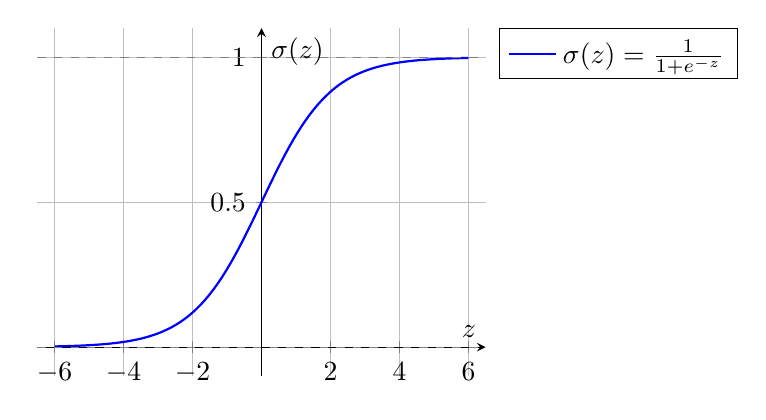
\begin{tikzpicture}
      \begin{axis}[
          width=0.6\textwidth,
          height=6cm,
          axis lines=middle,
          xlabel={$z$},
          ylabel={$\sigma(z)$},
          grid=major,
          ymin=-0.1, ymax=1.1,
          xmin=-6.5, xmax=6.5,
          samples=100,
          domain=-6:6,
          legend pos=outer north east
        ]
        \addplot [blue, thick] {1/(1+exp(-x))};
        \addlegendentry{$\sigma(z) = \frac{1}{1+e^{-z}}$}
        \addplot [dashed, gray, domain=-6.5:6.5] {0};
        \addplot [dashed, gray, domain=-6.5:6.5] {1};
      \end{axis}
    \end{tikzpicture}
    \caption[Sigmoid Activation Function]{The Sigmoid activation function.}
    \label{fig:sigmoid_plot}
    \caption*{Author's illustration.}
  \end{figure}


  \paragraph{Hyperbolic Tangent Function (\( \tanh \))}
  The hyperbolic tangent function maps any real input to the range (-1, 1). It is defined as:
  \begin{equation}
    \tanh(z) = \frac{e^z - e^{-z}}{e^z + e^{-z}} = 2\sigma(2z) - 1
  \end{equation}
  It is frequently used as the main activation function for hidden states in RNNs and LSTMs (see main text, e.g., Equations~\ref{eq:rnn_hidden_state}, \ref{eq:lstm-candidate-cell}, \ref{eq:lstm-hidden-state}). See Figure~\ref{fig:tanh_plot}.

  \begin{figure}[htbp]
    \centering
    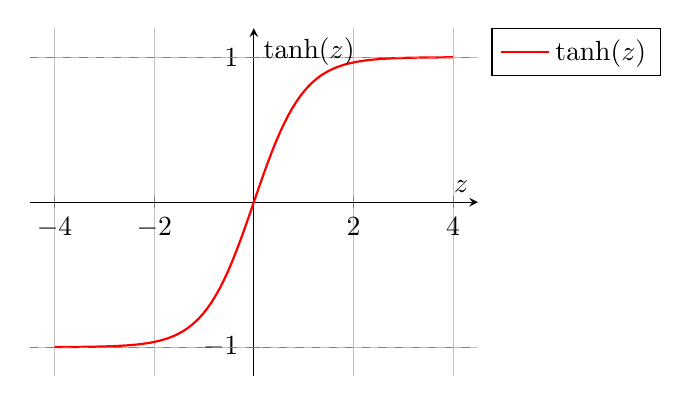
\begin{tikzpicture}
      \begin{axis}[
          width=0.6\textwidth,
          height=6cm,
          axis lines=middle,
          xlabel={$z$},
          ylabel={$\tanh(z)$},
          grid=major,
          ymin=-1.2, ymax=1.2,
          xmin=-4.5, xmax=4.5,
          samples=100,
          domain=-4:4,
          legend pos=outer north east
        ]
        \addplot [red, thick] {tanh(x)};
        \addlegendentry{$\tanh(z)$}
        \addplot [dashed, gray, domain=-4.5:4.5] {-1};
        \addplot [dashed, gray, domain=-4.5:4.5] {1};
      \end{axis}
    \end{tikzpicture}
    \caption[Tanh activation function]{The Hyperbolic Tangent (tanh) activation function.}
    \label{fig:tanh_plot}
    \caption*{Author's illustration.}
  \end{figure}


  \paragraph{Rectified Linear Unit (ReLU)}
  The ReLU function outputs the input directly if it is positive, and zero otherwise. It is defined as:
  \begin{equation}
    \text{ReLU}(z) = \max(0, z)
  \end{equation}
  ReLU is widely used in deep learning due to its simplicity and effectiveness in mitigating the vanishing gradient problem for positive inputs. It is used within the model presented in this thesis (see main text, e.g., Section~\ref{sec:integrated_architecture}). See Figure~\ref{fig:relu_plot}.

  \begin{figure}[htbp]
    \centering
    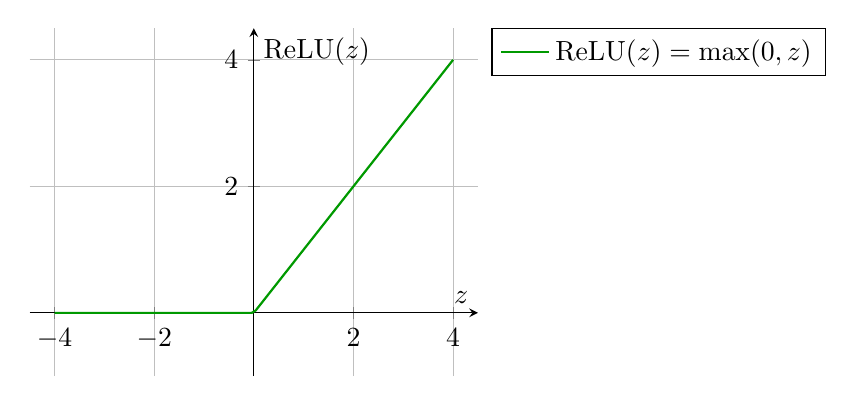
\begin{tikzpicture}
      \begin{axis}[
          width=0.6\textwidth,
          height=6cm,
          axis lines=middle,
          xlabel={$z$},
          ylabel={ReLU$(z)$},
          grid=major,
          ymin=-1, ymax=4.5,
          xmin=-4.5, xmax=4.5,
          samples=100,
          legend pos=outer north east
        ]
        \addplot [green!60!black, thick, domain=-4:4] {max(0,x)};
        \addlegendentry{ReLU$(z) = \max(0, z)$}
      \end{axis}
    \end{tikzpicture}
    \caption[ReLU activation function]{The Rectified Linear Unit (ReLU) activation function.}
    \label{fig:relu_plot}
    \caption*{Author's illustration.}
  \end{figure}


  \paragraph{Softmax Function}
  The softmax function converts a vector of K real numbers \( \bm{z} = (z_1, ..., z_K) \) into a probability distribution consisting of K probabilities. The function is applied to the entire vector and the $i$-th element of the output vector is calculated as:
  \begin{equation}
    \text{softmax}(\bm{z})_i = \frac{e^{z_i}}{\sum_{j=1}^K e^{z_j}} \quad \text{for } i = 1, ..., K
  \end{equation}
  The outputs are non-negative and sum to 1 (\( \sum_{i=1}^K \text{softmax}(\bm{z})_i = 1 \)). Softmax is commonly used in the output layer of multi-class classification models and plays a crucial role in normalizing scores into attention weights in the Attention mechanism (see main text, e.g., Equation~\ref{eq:scaled_dot_product_attention}).

  \subsection{Distance and Similarity Metrics}
  \label{subsec:distance_metrics}
  These metrics quantify the difference or similarity between vectors, which is fundamental in many machine learning tasks. Let \( \bm{a}, \bm{b} \in \mathbb{R}^d \) be two vectors of dimension $d$.

  \paragraph{Euclidean Distance (L2 Distance)}
  \label{eq:euclidean_distance}
  The most common distance measure:
  \begin{equation}
    d_{\text{Euclidean}}(\bm{a}, \bm{b}) = ||\bm{a} - \bm{b}||_2 = \sqrt{\sum_{i=1}^d (a_i - b_i)^2}
  \end{equation}

  \paragraph{Manhattan Distance (L1 Distance)}
  Measures distance along axes at right angles:
  \begin{equation}
    d_{\text{Manhattan}}(\bm{a}, \bm{b}) = ||\bm{a} - \bm{b}||_1 = \sum_{i=1}^d |a_i - b_i|
  \end{equation}

  \paragraph{Cosine Similarity}
  Measures the cosine of the angle between vectors:
  \begin{equation}
    \text{CosineSimilarity}(\bm{a}, \bm{b}) = \frac{\bm{a} \cdot \bm{b}}{||\bm{a}||_2 ||\bm{b}||_2} = \frac{\sum_{i=1}^d a_i b_i}{\sqrt{\sum_{i=1}^d a_i^2} \sqrt{\sum_{i=1}^d b_i^2}}
  \end{equation}
  Widely used for high-dimensional vectors. Cosine Distance is sometimes defined as $ 1 - \text{CosineSimilarity}(\bm{a}, \bm{b}) $.

  \subsection{Neural Network Techniques}
  \label{subsec:nn_techniques_app}

  \paragraph{Attention Mechanism Components}
  The Scaled Dot-Product Attention mechanism relies on:
  \begin{itemize}
    \item \textit{Dot Product Similarity} Compatibility between query $ \bm{q} $ and key $ \bm{k} $ often computed as $ \bm{q}^T \bm{k} $. Matrix product $ QK^T $ computes pairwise dot products.
    \item \textit{Scaling} Scores $ QK^T $ are divided by $ \sqrt{d_k} $ before softmax to stabilize gradients, especially for large $ d_k $.
  \end{itemize}

  \paragraph{Normalization Techniques}
  Help stabilize training and improve convergence.
  \begin{itemize}
    \item \textit{Layer Normalization (LayerNorm)} Normalizes inputs across features for each individual data sample. Computation is independent of batch size. For input vector $ \bm{x} $:
          \begin{equation}
            \text{LayerNorm}(\bm{x}) = \bm{\gamma} \odot \frac{\bm{x} - \mu_{\text{sample}}}{\sqrt{\sigma^2_{\text{sample}} + \epsilon}} + \bm{\beta}
            \label{eq:layernorm}
          \end{equation}
          $ \mu_{\text{sample}} $, $ \sigma^2_{\text{sample}} $ are mean/variance across features of $ \bm{x} $. $ \bm{\gamma}, \bm{\beta} $ are learnable scale/shift parameters. Frequently used in RNNs and Transformers (used in this thesis).
    \item \textit{Batch Normalization (BatchNorm)} (Included for contrast) Normalizes across the batch dimension for each feature. Effective in CNNs, but dependence on batch statistics can be less suitable for sequence models.
  \end{itemize}

  \paragraph{Pooling Strategies for Sequences}
  Aggregate information across the sequence dimension $ H = [\bm{h}_1, \bm{h}_2, ..., \bm{h}_T] $, where $ \bm{h}_t \in \mathbb{R}^d $.
  \begin{itemize}
    \item \textit{Mean Pooling} Calculates element-wise average:
          \begin{equation}
            \bm{h}_{\text{mean\_pool}} = \frac{1}{T} \sum_{t=1}^T \bm{h}_t
          \end{equation}
          Result $ \bm{h}_{\text{mean\_pool}} \in \mathbb{R}^d $ represents average activation. Used in this thesis.
    \item \textit{Max Pooling} Calculates element-wise maximum:
          \begin{equation}
            (\bm{h}_{\text{max\_pool}})_j = \max_{t=1...T} (\bm{h}_t)_j \quad \text{for } j = 1, ..., d
          \end{equation}
          Result $ \bm{h}_{\text{max\_pool}} \in \mathbb{R}^d $ captures strongest activation per feature.
  \end{itemize}

  \paragraph{Weight Initialization} Crucial for effective training.
  \begin{itemize}
    \item \textit{Kaiming (He) Initialization} For ReLU layers \autocite{he2015delving}. Aims to keep variance constant. Kaiming Normal init draws weights from $ \mathcal{N}(0, \text{std}^2) $ with:
          \begin{equation}
            \text{std} = \sqrt{\frac{2}{\text{fan\_in}}}
          \end{equation}
          `fan\_in` is the number of input units. Used in this thesis.
    \item \textit{Xavier (Glorot) Initialization} For symmetric activations (tanh, sigmoid) \autocite{glorot2010understanding}. Aims to keep variance constant across layers. Xavier Normal init uses:
          \begin{equation}
            \text{std} = \sqrt{\frac{2}{\text{fan\_in} + \text{fan\_out}}}
          \end{equation}
          `fan\_out` is the number of output units.
  \end{itemize}

  \paragraph{Regularization Techniques} Prevent overfitting.
  \begin{itemize}
    \item \textit{L2 Regularization (Weight Decay)} Adds penalty to loss function proportional to squared magnitude of weights $ \theta $:
          \begin{equation}
            J_{reg}(\theta) = J(\theta) + \frac{\lambda}{2} ||\theta||_2^2 = J(\theta) + \frac{\lambda}{2} \sum_i \theta_i^2
          \end{equation}
          $ \lambda $ is regularization strength. Encourages smaller weights.
    \item \textit{Dropout} Randomly sets a fraction of neuron activations to zero during training \autocite{srivastava2014dropout}. Prevents co-adaptation. Dropout rate specifies the zeroing probability. Used in this thesis (LSTM layers and fully connected block).
  \end{itemize}

  \paragraph{Data Handling for Sequences}
  \begin{itemize}
    \item \textit{Sequence Padding} Augments shorter sequences in a batch with padding values (often zero) to match the longest sequence, creating uniform tensors. `collate\_fn` in this thesis uses `pad\_sequence`. Important to mask padded values in subsequent computations (loss, attention).
  \end{itemize}


  \subsection{Optimization Algorithms}
  \label{subsec:optimization_app}
  Update model parameters $ \theta $ to minimize loss $ J(\theta) $.

  \paragraph{Stochastic Gradient Descent (SGD)}
  Fundamental algorithm updating parameters based on mini-batch gradient:
  \begin{equation}
    \theta_{k+1} = \theta_k - \eta \nabla J(\theta_k; \bm{x}^{(i)}; \bm{y}^{(i)})
  \end{equation}
  $ \eta $ is learning rate. Variants include momentum.

  \paragraph{Adam Optimizer}
  Adaptive learning rate algorithm using first and second moment estimates of gradients \autocite{kingma2014adam}. Computes biased moments ($ \bm{m}_t, \bm{v}_t $), bias-corrected moments ($ \hat{\bm{m}}_t, \hat{\bm{v}}_t $), and updates:
  \begin{equation}
    \theta_{t+1} = \theta_t - \frac{\eta}{\sqrt{\hat{\bm{v}}_t} + \epsilon} \hat{\bm{m}}_t
    \label{eq:adam}
  \end{equation}
  Used for training the model in this work.

  \paragraph{Learning Rate Scheduling}
  Adjust $ \eta $ during training to improve convergence.
  \begin{itemize}
    \item \textit{ReduceLROnPlateau} Reduces $ \eta $ if a monitored metric (e.g., validation loss) stops improving for 'patience' epochs. Employed in this thesis.
    \item \textit{Step Decay} Reduces $ \eta $ by fixed factor every N epochs.
    \item \textit{Cosine Annealing} Decreases $ \eta $ following a cosine curve.
  \end{itemize}

  \subsection{Loss Functions and Metrics}
  \label{subsec:loss_metrics_app}
  Quantify the difference between predictions and true values.

  \paragraph{Binary Cross-Entropy (BCE)}
  \label{eq:bce}
  For binary classification tasks ($y_i \in \{0, 1\}$, prediction $\hat{p}_i$). Loss function used in this thesis.
  \begin{equation}
    \text{BCE} = -\frac{1}{N} \sum_{i=1}^N [ y_i \log(\hat{p}_i) + (1 - y_i) \log(1 - \hat{p}_i) ]
  \end{equation}

  \paragraph{Regression Metrics}
  For evaluating models predicting continuous variables.
  \begin{itemize}
    \item \textit{Mean Squared Error (MSE)} Average of squared differences. Sensitive to outliers \autocite{fahrmeir2016statistik}.
          \begin{equation}
            \text{MSE} = \frac{1}{n} \sum_{i=1}^{n} (y_i - \hat{y}_i)^2
          \end{equation}
    \item \textit{Mean Absolute Error (MAE)} Average of absolute differences. More robust to outliers \autocite{fahrmeir2016statistik}.
          \begin{equation}
            \text{MAE} = \frac{1}{n} \sum_{i=1}^{n} |y_i - \hat{y}_i|
          \end{equation}
    \item \textit{Mean Absolute Percentage Error (MAPE)} Average percentage difference. Useful when scale varies.
          \begin{equation}
            \text{MAPE} = \frac{1}{n} \sum_{i=1}^{n} \left| \frac{y_i - \hat{y}_i}{y_i} \right| \times 100\%
          \end{equation}
  \end{itemize}


  \subsection{Decision Tree Splitting Criteria}
  \label{subsec:decision_tree_splitting_criteria}

  \paragraph{Gini Impurity}
  Measures the probability of incorrect classification if a randomly chosen sample from the node were randomly labeled according to the class distribution at the node. For $K$ classes ($K = 2$ here), with $p_k$ being the proportion of samples of class $k$ in set $S$:
  \begin{equation}
    G(S) = 1 - \sum_{k=1}^{K} p_k^2
    \label{eq:gini_impurity}
  \end{equation}
  A lower Gini impurity indicates a purer node. Split quality (dividing $S$ into $S_{left}$, $S_{right}$) is evaluated by weighted average impurity:
  \begin{equation}
    \text{Gini}_{\text{split}}(S) = \frac{|S_{left}|}{|S|} G(S_{left}) + \frac{|S_{right}|}{|S|} G(S_{right})
    \label{eq:gini_split}
  \end{equation}
  The DTree seeks splits that minimize this value \autocite{breiman1984classification}.


  \chapter{Statistical Validation Methodology}
  \label{app:cct}

  This chapter details the statistical tests used for combining results across multiple runs and assessing overall significance, complementing the permutation testing described in the main text (e.g., \autoref{sec:permtest}).

  \section{Cauchy Combination Test (CCT)}
  \label{sec:cct_methodology}

  The Cauchy Combination Test \autocite{liu2020cauchy} provides a powerful method for combining $k$ individual p-values, $p_1, p_2, ..., p_k$, obtained from multiple statistical tests (in this case, the $k=10$ runs of the permutation test for each feature subset) into a single overall p-value. A key advantage of the CCT is its robustness under arbitrary dependence structures among the individual p-values.

  The CCT transforms each individual p-value $p_i$ using the inverse CDF of the standard Cauchy distribution ($C(0,1)$), equivalent to using the tangent function:
  \begin{equation}
    t_i = \tan\left( (0.5 - p_i) \pi \right)
    \label{eq:cct_transform}
  \end{equation}
  The combined test statistic, $T_{CCT}$, is the mean (assuming equal weights $w_i=1/k$) of these transformed values:
  \begin{equation}
    T_{CCT} = \frac{1}{k} \sum_{i=1}^k t_i = \frac{1}{k} \sum_{i=1}^k \tan\left( (0.5 - p_i) \pi \right)
    \label{eq:cct_statistic}
  \end{equation}
  Under the global null hypothesis, $T_{CCT}$ approximately follows a standard Cauchy distribution, $C(0,1)$.

  The final combined p-value, $P_{CCT}$, is the upper tail probability:
  \begin{equation}
    P_{CCT} = P(C(0,1) \ge T_{CCT}) = 1 - F_{C(0,1)}(T_{CCT}) = 0.5 - \frac{\arctan(T_{CCT})}{\pi}
    \label{eq:cct_pvalue}
  \end{equation}
  where $F_{C(0,1)}$ is the CDF of the standard Cauchy distribution. A small $P_{CCT}$ indicates strong evidence against the global null. The CCT is powerful when the signal is sparse and robust to dependence.

  \section{Binomial Test for Rejection Rate}
  \label{sec:binom_test_methodology}

  The Binomial test formally assesses the significance of the observed \textit{Rejection Rate} ($RR$) \autocite{fahrmeir2016statistik}, defined as the proportion of $k$ runs where the null hypothesis $H_0$ was rejected at significance level $\alpha$. $RR = k_{obs}/k$, where $k_{obs}$ is the observed number of rejections ($p_{run} < \alpha$).

  The test addresses: "Is $k_{obs}$ significantly greater than expected by chance if $H_0$ were true for all runs?"

  The null hypothesis ($H_0$) for the Binomial test is that the true probability of rejecting in a single run is $\alpha$. Under $H_0$, the number of rejections $X$ follows a Binomial distribution:
  \begin{equation}
    X \sim B(k, \alpha)
  \end{equation}
  The probability mass function (PMF) is:
  \begin{equation}
    P(X=i | k, \alpha) = \binom{k}{i} \alpha^i (1-\alpha)^{k-i}
    \label{eq:binom_pmf}
  \end{equation}
  The p-value for observing $k_{obs}$ or more rejections (one-sided test) is:
  \begin{equation}
    P_{Binom} = P(X \ge k_{obs} | H_0) = \sum_{i=k_{obs}}^{k} P(X=i | k, \alpha) = \sum_{i=k_{obs}}^{k} \binom{k}{i} \alpha^i (1-\alpha)^{k-i}
    \label{eq:binom_pvalue}
  \end{equation}
  A small $P_{Binom}$ suggests the observed $RR$ is significantly higher than expected by chance. This complements methods like CCT by focusing on the consistency of rejection.


  \chapter{Detailed Validation Results}
  \label{app:detailed_results}

  This chapter presents the detailed numerical results from the statistical validation analyses discussed in \autoref{app:cct}.

  \section{Decision Tree Model Results}
  \label{sec:dt_results_appendix}

  The following table presents the detailed hypothesis testing results obtained using the DTree as the model for distinguishing between real and simulated data. The evaluation metric was the ROC AUC score. The results are based on $k=10$ independent runs, each employing $N=1000$ permutations for p-value calculation. The significance level for individual run rejection and the Binomial test was set at $\alpha=0.05$. The Cauchy Combination Test (CCT) was used to combine p-values across runs (yielding $P_{CCT}$), and the Binomial test assessed the significance of the observed Rejection Rate ($RR$, yielding $P_{Binom}$).

  \begin{table}[htbp]
    \centering
    \caption[Detailed Decision Tree Model Results applying CCT]{Detailed Decision Tree validation results across 10 runs (N=1000, $\alpha=0.05$).}
    \label{tab:results-dt-appendix}
    \resizebox{\textwidth}{!}{%
      \begin{tabular}{l c c c c c p{3cm}}
        \toprule
        \textbf{Component ($\mathcal{F}_c$)} & \textbf{$\overline{\text{ROC AUC}}$} & \textbf{$\sigma_{\text{ROC AUC}}$} & \textbf{$P_{CCT}$} & \textbf{RR} & \textbf{$P_{Binom}$} & \textbf{Assessment} \\
        \midrule
        \texttt{time\_model}                 & 1.0000                               & 0.0000                             & 0.0000             & 1.00        & 0.0000               & INACCURATE          \\
        \texttt{resource\_model}             & 0.9817                               & 0.0088                             & 0.0000             & 1.00        & 0.0000               & INACCURATE          \\
        \texttt{transformation\_model}       & 1.0000                               & 0.0000                             & 0.0000             & 1.00        & 0.0000               & INACCURATE          \\
        \texttt{transition\_model}           & 1.0000                               & 0.0000                             & 0.0000             & 1.00        & 0.0000               & INACCURATE          \\
        \texttt{process\_model}              & 1.0000                               & 0.0000                             & 0.0000             & 1.00        & 0.0000               & INACCURATE          \\
        \texttt{kpi\_based}                  & 1.0000                               & 0.0000                             & 0.0000             & 1.00        & 0.0000               & INACCURATE          \\
        \texttt{all\_features}               & 1.0000                               & 0.0000                             & 0.0000             & 1.00        & 0.0000               & INACCURATE          \\
        \bottomrule
      \end{tabular}%
    }
    \caption*{Source: Author's tabulation based on permutation test results.}
  \end{table}

  As evidenced by the results in Table \ref{tab:results-dt-appendix}, both the Cauchy Combination Test ($P_{CCT}=0.0000$) and the Binomial test ($P_{Binom}=0.0000$) yielded extremely significant p-values for all feature subsets when using the Decision Tree model at $\alpha=0.05$. The perfect rejection rate ($RR=1.00$) across all components further underscores this. This indicates a highly consistent and statistically robust ability of the DT model to distinguish between the real and simulated data across all evaluated components based on the engineered features, leading to the assessment "INACCURATE" for all components according to the defined validation framework.

  \section{BiLSTM Model Results}
  \label{sec:lstm_results_appendix}

  The following table presents the detailed hypothesis testing results obtained using the BiLSTM classifier as the blackbox model for distinguishing between real and simulated data. The evaluation metric was the ROC AUC score. The results are based on $k=10$ independent runs, each employing $N=1000$ permutations for p-value calculation. The significance level for individual run rejection and the Binomial test was set at $\alpha=0.01$. The Cauchy Combination Test (CCT) was used to combine p-values across runs (yielding $P_{CCT}$), and the Binomial test assessed the significance of the observed Rejection Rate ($RR$, yielding $P_{Binom}$).

  \begin{table}[htbp]
    \centering
    \caption[Detailed BiLSTM Model Results]{Detailed BiLSTM validation results across 10 runs (N=1000, $\alpha=0.01$).}
    \label{tab:results-lstm-appendix}
    \resizebox{\textwidth}{!}{%
      \begin{tabular}{l l l l l l p{3cm}}
        \toprule
        \textbf{Component ($\mathcal{F}_c$)} & \textbf{$\overline{\text{ROC AUC}}$} & \textbf{$\sigma_{\text{ROC AUC}}$} & \textbf{$P_{CCT}$} & \textbf{RR} & \textbf{$P_{Binom}$} & \textbf{Assessment} \\
        \midrule
        \texttt{time\_model}                 & 1.0000                               & 0.0000                             & 0.0000             & 1.00        & 0.0000               & INACCURATE          \\
        \texttt{resource\_model}             & 0.9945                               & 0.0071                             & 0.0000             & 1.00        & 0.0000               & INACCURATE          \\
        \texttt{transformation\_model}       & 1.0000                               & 0.0000                             & 0.0000             & 1.00        & 0.0000               & INACCURATE          \\
        \texttt{transition\_model}           & 0.9644                               & 0.1067                             & 0.0000             & 1.00        & 0.0000               & INACCURATE          \\
        \texttt{process\_model}              & 0.9714                               & 0.0858                             & 0.0000             & 1.00        & 0.0000               & INACCURATE          \\
        \texttt{kpi\_based}                  & 0.9975                               & 0.0054                             & 0.0000             & 1.00        & 0.0000               & INACCURATE          \\
        \texttt{all\_features}               & 1.0000                               & 0.0000                             & 0.0000             & 1.00        & 0.0000               & INACCURATE          \\
        \bottomrule
      \end{tabular}%
    }
    \caption*{Source: Author's tabulation based on permutation test results.}
  \end{table}

  As shown in Table \ref{tab:results-lstm-appendix}, the results for the BiLSTM model are the same observed with the DTree. Using the stricter significance level of $\alpha=0.01$, both the CCT ($P_{CCT}=0.0000$) and the Binomial test ($P_{Binom}=0.0000$) yielded extremely significant p-values for all feature subsets. The rejection rate was also perfect ($RR=1.00$) across all components. This demonstrates a consistent and statistically robust capability of the BiLSTM model to distinguish between the real and simulated data across all SBDT components evaluated, leading to the assessment "INACCURATE" for all components within the validation framework.


  \chapter{Supplementary Figures}
  \label{app:supp_figures}

  \section{Design Science Research Methodology}
  \label{app:dsr_figure}
  \begin{figure}[htbp]
    \centering
    \includegraphics[width=0.6\textwidth]{figures/dsr.png}
    \caption[Design Science Methodology]{The cyclical design science research model. The model consists of six steps. The problem identification (1) refers to the research gap in automated \gls{vvuq} of \gls{sbdt}. Defining the solution objectives (2) specifies the research gap by formulating questions and hypotheses based on the theoretical foundations. The design and development (3) phase includes the development of the framework. The demonstration (4) phase shows the application of the framework in a case study. The evaluation (5) phase assesses the effectiveness of the framework. The communication (6) phase concludes the research by presenting the results.}
    \label{fig:DSR}
    \caption*{Illustration based on \textcite{peffers2007design}}
  \end{figure}

  \section{Time Encoding on Unit Circle}
  \label{app:time_encoding_figure}
  \begin{figure}[htbp]
    \centering
    \begin{tikzpicture}[
        scale=3,
        hour dot/.style={circle, fill=blue!70, inner sep=1.5pt},
        hour label/.style={font=\small}
      ]

      \draw [gray, dashed] (0,0) circle (1);

      \draw [->, gray!80] (-1.3,0) -- (1.3,0) node[right, black] {$x_{\cos}$};
      \draw [->, gray!80] (0,-1.3) -- (0,1.3) node[above, black] {$x_{\sin}$};
      \node[above=5pt] at (current bounding box.north) {Hour of Day Encoded on Unit Circle};


      \foreach \h in {0,...,23} {
          \pgfmathsetmacro{\angle}{\h * 360 / 24}

          \node[hour dot] at (\angle:1) {};

          \ifnum \h = 0 \node[hour label, anchor=west] at (\angle:1.15) {0h (Midnight)}; \fi
          \ifnum \h = 3 \node[hour label, anchor=south west] at (\angle:1.15) {3h}; \fi
          \ifnum \h = 6 \node[hour label, anchor=south] at (\angle:1.15) {6h (Morning)}; \fi
          \ifnum \h = 9 \node[hour label, anchor=south east] at (\angle:1.15) {9h}; \fi
          \ifnum \h = 12 \node[hour label, anchor=east] at (\angle:1.15) {12h (Noon)}; \fi
          \ifnum \h = 15 \node[hour label, anchor=north east] at (\angle:1.15) {15h}; \fi
          \ifnum \h = 18 \node[hour label, anchor=north] at (\angle:1.15) {18h (Evening)}; \fi
          \ifnum \h = 21 \node[hour label, anchor=north west] at (\angle:1.15) {21h}; \fi
        }

    \end{tikzpicture}
    \caption[Feature Transformation]{Sine and Cosine transformation of the hour of the day (0-23). Each hour is mapped to a point $(x_{\cos}, x_{\sin})$ on the unit circle (blue dots). Key hours are labelled, demonstrating how the transformation preserves cyclical continuity (hour 23 is near hour 0).}
    \label{fig:time-encoding}
    \caption*{Source: Author's illustration}
  \end{figure}

\end{appendices}

%------------------------------------------------------------------------
% Bibliography
%------------------------------------------------------------------------
\printbibliography

\end{document}
